\documentclass[12pt,a4paper]{report}
\usepackage{fontspec}
\usepackage{polyglossia}
\setmainlanguage{vietnamese}
\setmainfont{TeX Gyre Termes}
\setsansfont{TeX Gyre Heros}
\setmonofont{TeX Gyre Cursor}[Scale=0.88]

\usepackage[a4paper,left=3cm,right=2cm,top=2.5cm,bottom=2.5cm,headheight=15pt]{geometry}
\usepackage{etoolbox}
\usepackage{graphicx,booktabs,longtable,array,float,xcolor,amsmath,enumitem,tabularx}
\usepackage{caption}
\usepackage{titlesec}
\usepackage{tocloft}
\usepackage{fancyhdr}
\usepackage{listings}
\usepackage{tikz}
\usetikzlibrary{arrows.meta,positioning,shapes.geometric,calc}
\usepackage[unicode,hidelinks,pdftitle={Báo cáo phân tích dữ liệu giá nhà Melbourne}]{hyperref}
\usepackage{xurl}

\linespread{1.2}
\emergencystretch=3em
\setlength{\parindent}{0pt}
\setlength{\parskip}{6pt plus 1pt minus 0.5pt}
\setlist{leftmargin=1.6em,labelsep=0.6em,itemsep=2pt,parsep=0pt,topsep=2pt,partopsep=0pt}
\setlist[enumerate]{leftmargin=1.8em}
\setlength{\tabcolsep}{5pt}
\renewcommand{\arraystretch}{1.15}
\newcolumntype{L}[1]{>{\raggedright\arraybackslash}p{#1}}
\graphicspath{{../outputs/}}

\gappto\captionsvietnamese{%
  \renewcommand{\contentsname}{Mục lục}%
  \renewcommand{\listfigurename}{Danh mục hình}%
  \renewcommand{\listtablename}{Danh mục bảng}}

% ---------- tiêu đề chương: "Chương 1. Giới thiệu", phụ lục: "Phụ lục A. ..." ----------
\titleformat{\chapter}[hang]{\normalfont\Large\bfseries}{\chaptertitlename\ \thechapter.}{0.5em}{}
\titleformat{name=\chapter,numberless}[hang]{\normalfont\Large\bfseries}{}{0pt}{}
\titlespacing*{\chapter}{0pt}{-10pt}{18pt}
\titleformat{\section}{\normalfont\large\bfseries}{\thesection.}{0.5em}{}
\titleformat{\subsection}{\normalfont\normalsize\bfseries}{\thesubsection.}{0.5em}{}
\titleformat{\paragraph}[runin]{\normalfont\bfseries}{}{0pt}{}
\titlespacing*{\section}{0pt}{16pt plus 2pt}{6pt}
\titlespacing*{\subsection}{0pt}{12pt plus 2pt}{4pt}
\titlespacing*{\paragraph}{0pt}{8pt}{0.4em}

% ---------- mục lục ----------
\renewcommand{\cftchappresnum}{Chương }
\renewcommand{\cftchapaftersnum}{.}
\setlength{\cftchapnumwidth}{5.6em}
\setlength{\cftsecindent}{5.6em}
\setlength{\cftsecnumwidth}{3em}
\setlength{\cftsubsecindent}{8.6em}
\setlength{\cftsubsecnumwidth}{3.4em}
\setlength{\cftbeforechapskip}{0.6em}
\renewcommand{\cftchapfont}{\bfseries}
\renewcommand{\cftchappagefont}{\bfseries}
\makeatletter
\newcommand{\danhmuc}[3]{\chapter*{#2}\markboth{#2}{}#3\@starttoc{#1}}
\makeatother
\setlength{\cftfignumwidth}{2.4em}
\setlength{\cfttabnumwidth}{2.4em}
\pagestyle{fancy}
\fancyhf{}
\fancyhead[L]{\small\itshape\leftmark}
\fancyfoot[C]{\thepage}
\renewcommand{\headrulewidth}{0.4pt}
\renewcommand{\chaptermark}[1]{\markboth{\chaptertitlename\ \thechapter.\ #1}{}}
\fancypagestyle{plain}{\fancyhf{}\fancyfoot[C]{\thepage}\renewcommand{\headrulewidth}{0pt}}

% ---------- hình, bảng, mã ----------
\captionsetup{font=small,labelfont=bf,labelsep=period,justification=centering,singlelinecheck=false,width=0.92\linewidth}
\captionsetup[table]{skip=6pt}
% Lưu ý: khối mã (lstlisting) chỉ dùng ký tự ASCII, vì gói listings làm đảo chữ có dấu tiếng Việt khi dịch bằng XeLaTeX; chú thích tiếng Việt viết ở phần văn bản.
\lstset{basicstyle=\ttfamily\footnotesize,breaklines=true,frame=single,language=Python,columns=fullflexible,
        keywordstyle=\bfseries,commentstyle=\itshape\color{gray},showstringspaces=false,xleftmargin=4pt,xrightmargin=4pt,framesep=4pt,aboveskip=6pt,belowskip=6pt}

% Khung giữ chỗ cho ảnh chụp màn hình thật: chưa có tệp thì hiện khung ghi tên tệp cần chèn (không dùng ảnh giả).
\newcommand{\anhchup}[3]{%
  \begin{figure}[H]\centering
  \IfFileExists{screenshots/#1}%
    {\includegraphics[width=0.95\linewidth]{screenshots/#1}}%
    {\fbox{\parbox[c][5.5cm][c]{0.85\linewidth}{\centering\textit{Khung giữ chỗ: chèn ảnh chụp màn hình\\[2pt]\texttt{screenshots/\detokenize{#1}}}}}}%
  \caption{#2}\label{#3}\end{figure}}

% ---------- thông tin bìa  ----------
% Ghi nguon so lieu duoi bang/hinh/doan van
\newcommand{\nguon}[1]{\par\smallskip\noindent{\footnotesize\raggedright\emph{Nguồn:} #1\par}}
\emergencystretch=3em
\DeclareRobustCommand{\_}{\textunderscore\allowbreak{}}
\newcommand{\bs}[1]{\texttt{outputs/report\_metrics.csv} (mã #1)}
\newcommand{\bm}[1]{\texttt{outputs/model\_error\_metrics.csv} (mã #1)}
\newcommand{\TenTruong}{{Trường Đại học Sư Phạm TPHCM}}
\newcommand{\TenKhoa}{{Khoa Công nghệ Thông tin}}
\newcommand{\HoTen}{{Nguyễn Tuấn Khải}}
\newcommand{\MSSV}{{51.01.104.125}}
\newcommand{\GiangVien}{{ThS. Lương Trần Hy Hiến}}
\newcommand{\NamHoc}{2026 - 2027}

\emergencystretch=2em
\begin{document}
\pagenumbering{gobble}
\begin{titlepage}
\centering
{\large \textbf{\TenTruong}}\\[2pt]
{\large \TenKhoa}\\[2.5cm]
{\Large \textbf{BÁO CÁO ĐỒ ÁN}}\\[4pt]
{\large Môn học: Lập trình Python}\\[2cm]
{\Large \textbf{ỨNG DỤNG DỰ ĐOÁN GIÁ BẰNG MACHINE LEARNING}}\\[6pt]
{\Large Phân tích dữ liệu giá nhà Melbourne}\\[3.5cm]
\begin{tabular}{rl}
Sinh viên thực hiện: & \HoTen\\[4pt]
Mã số sinh viên: & \MSSV\\[4pt]
Giảng viên hướng dẫn: & \GiangVien\\
\end{tabular}\\[\fill]
Năm \NamHoc
\end{titlepage}

\clearpage
\pagenumbering{roman}
\setcounter{page}{1}
\danhmuc{toc}{\contentsname}{}
\danhmuc{lof}{\listfigurename}{\addcontentsline{toc}{chapter}{\listfigurename}}
\danhmuc{lot}{\listtablename}{\addcontentsline{toc}{chapter}{\listtablename}}

\clearpage
\pagenumbering{arabic}
\setcounter{page}{1}
\chapter{Giới thiệu}

\section{Bối cảnh và mục tiêu}
Đề tài của môn Lập trình Python là \emph{Ứng dụng dự đoán giá bằng Machine Learning}. Báo cáo giữa kỳ thực hiện hai phần đầu của đề tài trên dữ liệu giao dịch nhà ở Melbourne (Úc): \emph{phân tích dữ liệu} (nguồn, kiểm tra, làm sạch, thống kê, trực quan hóa) và \emph{mô hình hồi quy} dự đoán giá bằng scikit-learn. Dữ liệu gồm 13,580 căn nhà bán từ 28/01/2016 đến 23/09/2017 (\bs{N01, N02}). Giao diện người dùng, cơ sở dữ liệu và phân quyền thuộc đồ án riêng, không nằm trong báo cáo này.

Các mục tiêu cụ thể:
\begin{enumerate}[nosep]
  \item Mô tả nguồn gốc, quy mô và ý nghĩa các cột của dữ liệu (Chương~\ref{ch:nguon}).
  \item Kiểm tra chất lượng dữ liệu và làm sạch bằng các quy tắc có lý do, có số dòng bị ảnh hưởng (Chương~\ref{ch:lamsach}).
  \item Thực hiện bảy phép phân tích thống kê gồm mục đích, phương pháp, kết quả và diễn giải (Chương~\ref{ch:phantich}).
  \item Trình bày năm biểu đồ thuộc năm dạng khác nhau (Chương~\ref{ch:trucquan}).
  \item Trình bày cơ sở lý thuyết của các thành phần scikit-learn được dùng: \texttt{Pipeline}, bộ tiền xử lý, Ridge, Random Forest, chia tập và chỉ số đánh giá (Chương~\ref{ch:lythuyet}).
  \item Huấn luyện, chọn và đánh giá mô hình hồi quy so với một mô hình cơ sở (baseline) (Chương~\ref{ch:mohinh}).
  \item Rút ra nhận xét có số liệu, nêu hạn chế và hướng cải thiện (Chương~\ref{ch:ketluan}).
\end{enumerate}

\section{Phạm vi và câu hỏi nghiên cứu}
\paragraph{Phạm vi.} Báo cáo chỉ dùng tệp \texttt{data/melb\_data.csv}. Mã nguồn gồm \texttt{pipeline.py} (kiểm tra, làm sạch, phân tích, biểu đồ), \texttt{train\_model.py} (huấn luyện và đánh giá mô hình) và notebook \texttt{melbourne\_\allowbreak data\_\allowbreak analysis\_\allowbreak pipeline.ipynb} (trình bày từng bước). Kết luận chỉ áp dụng cho Melbourne giai đoạn 2016--2017.

\paragraph{Nguồn số liệu.} Mọi số liệu trong báo cáo thuộc một trong ba loại. Loại thứ nhất là các tệp do \texttt{pipeline.py} và \texttt{train\_model.py} ghi vào \texttt{outputs/}. Loại thứ hai là các số tính thêm, do hàm \texttt{build\_report\_metrics()} (\texttt{pipeline.py}) và \texttt{build\_model\_error\_metrics()} (\texttt{train\_model.py}) ghi vào \texttt{outputs/report\_metrics.csv} và \texttt{outputs/model\_error\_metrics.csv} cùng biểu thức tính. Loại thứ ba là các kết quả đối chứng trong \texttt{outputs/doi\_chung/}. Dưới mỗi bảng và hình có dòng \emph{Nguồn} chỉ rõ tệp hoặc mã số liệu; Phụ lục~\ref{pl:nguon} tổng hợp cách tái lập.

\paragraph{Câu hỏi nghiên cứu.}
\begin{description}[leftmargin=2.2em,style=sameline,nosep]
  \item[Q1] Giá nhà phân phối thế nào, có lệch hoặc có ngoại lai đáng kể không? (Phép 1)
  \item[Q2] Giá khác nhau ra sao giữa các loại nhà, vùng và suburb? (Phép 2, 3, 5)
  \item[Q3] Số phòng và khoảng cách đến trung tâm ảnh hưởng đến giá thế nào? (Phép 4, 6)
  \item[Q4] Thuộc tính số nào tương quan mạnh nhất với giá, và ngoại lai làm sai lệch điều đó ra sao? (Phép 6)
  \item[Q5] Mô hình dự đoán tốt đến đâu so với baseline và yếu ở phân khúc nào? (Chương~\ref{ch:mohinh})
  \item[Q6] Vì sao mỗi thành phần scikit-learn được chọn và hoạt động thế nào? (Chương~\ref{ch:lythuyet})
  \item[Q7] Dữ liệu và cách làm có những hạn chế nào? (mục~\ref{sec:hanche})
\end{description}

\section{Công cụ và thư viện}
Toàn bộ xử lý viết bằng Python; các thư viện chính lấy từ \texttt{requirements.txt} (Bảng~\ref{tab:thuvien}).

\begin{table}[H]
\centering
\caption{Thư viện chính và vai trò trong dự án}\label{tab:thuvien}
\small
\begin{tabular}{@{}l L{6.2cm} L{4.6cm}@{}}
\toprule
Thư viện & Vai trò & Nơi dùng \\
\midrule
NumPy & Tính toán số, biến đổi \texttt{log1p} và ngược lại cho giá & \texttt{pipeline.py}, \texttt{train\_model.py} \\
Pandas & Đọc CSV, kiểm tra dữ liệu thiếu, \texttt{groupby}, \texttt{query}, tương quan & \texttt{pipeline.py}, notebook \\
scikit-learn & \texttt{Pipeline}, \texttt{ColumnTransformer}, \texttt{SimpleImputer}, \texttt{StandardScaler}, \texttt{OneHotEncoder}, \texttt{Ridge}, \texttt{RandomForestRegressor}, \texttt{DummyRegressor}, chia tập và các độ đo & \texttt{train\_model.py} \\
joblib & Lưu mô hình đã huấn luyện & \texttt{train\_model.py} \\
Matplotlib, Seaborn & Biểu đồ & \texttt{pipeline.py}, \texttt{train\_model.py} \\
Jupyter & Notebook trình bày các bước phân tích & \texttt{melbourne\_\allowbreak data\_\allowbreak analysis\_\allowbreak pipeline.ipynb} \\
\bottomrule
\end{tabular}
\nguon{\texttt{requirements.txt}; việc dùng thư viện trong từng tệp xem mã nguồn.}
\end{table}

\chapter{Nguồn dữ liệu}\label{ch:nguon}

\section{Tên bộ dữ liệu, nơi lấy, giấy phép, cách thu thập}\label{sec:nguon}
\begin{table}[H]
\centering
\caption{Thông tin nguồn của bộ dữ liệu}\label{tab:nguon}
\small
\begin{tabular}{@{}l L{10.2cm}@{}}
\toprule
Mục & Thông tin \\
\midrule
Tên bộ dữ liệu & \emph{Melbourne Housing Snapshot} \\
Nơi lấy & Kaggle, tài khoản đăng tải \texttt{dansbecker}; thông tin bộ dữ liệu tại \url{https://www.kaggle.com/datasets/dansbecker/melbourne-housing-snapshot} \\
Tệp sử dụng & \texttt{melb\_data.csv}, lưu trong \texttt{data/} \\
Giấy phép & CC BY-NC-SA 4.0 (Ghi công -- Phi thương mại -- Chia sẻ tương tự); cần giữ thông tin ghi công và tuân thủ điều kiện giấy phép khi chia sẻ hoặc biến đổi dữ liệu \\
Cách thu thập dữ liệu gốc & Bằng phương pháp cào dữ liệu web (web scraping) các tin đăng bán nhà công khai qua trang \url{https://www.domain.com.au}; bộ dữ liệu là bản chụp (snapshot) từ bộ Melbourne Housing của Tony Pino \\
Cách lấy dữ liệu trong dự án & Tải thủ công một tệp CSV từ Kaggle rồi đặt vào \texttt{data/}; dự án không tự cào dữ liệu hay gọi API để lấy bộ dữ liệu này. \\
\bottomrule
\end{tabular}
\end{table}

Mỗi dòng của tệp là một giao dịch bán nhà ở Melbourne (Úc), gồm vị trí, các thuộc tính của căn nhà, giá bán và ngày bán. Giá tính bằng đô la Úc (AUD).

Mọi số liệu trong báo cáo này chỉ tính trên tệp \texttt{melb\_data.csv}.

\section{Quy mô: số bản ghi, số thuộc tính, khoảng thời gian}\label{sec:quymo}
\begin{table}[H]
\centering
\caption{Quy mô và phạm vi của dữ liệu}\label{tab:quymo}
\small
\begin{tabular}{@{}l r@{}}
\toprule
Chỉ tiêu & Giá trị \\
\midrule
Số bản ghi (giao dịch) & 13,580 \\
Số thuộc tính (cột) trong tệp gốc & 21 \\
Số thuộc tính sau khi thêm biến dẫn xuất (\texttt{SaleMonth}, \texttt{HouseAge}) & 23 \\
Khoảng thời gian bán & 28/01/2016 -- 23/09/2017 \\
Số suburb & 314 \\
Số mã bưu chính (\texttt{Postcode}) & 198 \\
Số vùng (\texttt{Regionname}) & 8 \\
Số hội đồng quản lý (\texttt{CouncilArea}, chưa kể giá trị thiếu) & 33 \\
Số đại lý bán (\texttt{SellerG}) & 268 \\
Giá thấp nhất / cao nhất & 85,000 / 9,000,000 AUD \\
Giá trung vị / trung bình & 903,000 / 1,075,684 AUD \\
Số dòng trùng lặp hoàn toàn & 0 \\
\bottomrule
\end{tabular}
\end{table}

Bộ dữ liệu vượt xa quy mô tối thiểu mà đề tài yêu cầu (khoảng 500 bản ghi và 5 thuộc tính). Về cơ cấu, nhà riêng (\texttt{h}) chiếm 69.6\% số dòng (9,449 dòng), căn hộ (\texttt{u}) 22.2\% (3,017 dòng) và nhà liền kề (\texttt{t}) 8.2\% (1,114 dòng). Theo vùng, Southern Metropolitan chiếm 34.6\%, Northern Metropolitan 28.6\%, Western Metropolitan 21.7\% và Eastern Metropolitan 10.8\%; ba vùng Victoria (Eastern, Northern, Western) cộng lại chỉ có 126 dòng (0.9\%).

Về thời gian, dữ liệu trải trên 19 tháng có giao dịch nhưng không liên tục. Không có giao dịch nào trong tháng 3/2016 và tháng 1/2017; tháng 1/2016 chỉ có 2 giao dịch và tháng 2/2016 có 26 giao dịch, trong khi các tháng còn lại có từ 318 đến 1,536 giao dịch. Do đó quý 1/2016 gần như trống (28 giao dịch) và mọi so sánh theo thời gian cần đọc thận trọng (mục~\ref{sec:xuhuong}).

\section{Từ điển dữ liệu: ý nghĩa và kiểu từng cột}\label{sec:tudien}
Bảng~\ref{tab:tudien} mô tả 21 cột của tệp gốc. Ý nghĩa các cột theo cách hiểu thông dụng của bộ dữ liệu Melbourne Housing; đơn vị mét vuông của \texttt{Landsize} và \texttt{BuildingArea} được suy ra từ phân phối giá trị (trung vị sau làm sạch lần lượt là 533 và 126), vì tệp không kèm mô tả đơn vị. Tên hai cột \texttt{Lattitude} và \texttt{Longtitude} bị viết sai chính tả ngay từ tệp gốc và được giữ nguyên để không sửa dữ liệu thô.

{\small
\begin{longtable}{@{}l l L{6.6cm} L{3.1cm}@{}}
\caption{Từ điển dữ liệu của tệp \texttt{melb\_data.csv}}\label{tab:tudien}\\
\toprule
Cột & Kiểu & Ý nghĩa & Vai trò \\
\midrule
\endfirsthead
\toprule
Cột & Kiểu & Ý nghĩa & Vai trò \\
\midrule
\endhead
\midrule
\multicolumn{4}{r}{\emph{Tiếp ở trang sau}}\\
\endfoot
\bottomrule
\endlastfoot
\texttt{Suburb} & chuỗi & Tên suburb nơi căn nhà tọa lạc (314 giá trị) & Dùng, mã hóa mục tiêu \\
\texttt{Address} & chuỗi & Địa chỉ căn nhà; 13,378 giá trị khác nhau trên 13,580 dòng & Loại (gần như định danh) \\
\texttt{Rooms} & số nguyên & Số phòng (từ 1 đến 10) & Dùng \\
\texttt{Type} & chuỗi & Loại nhà: \texttt{h} nhà riêng, \texttt{t} nhà liền kề, \texttt{u} căn hộ (unit, duplex) & Dùng \\
\texttt{Price} & số thực & Giá bán, đơn vị AUD (85,000 đến 9,000,000) & Biến mục tiêu \\
\texttt{Method} & chuỗi & Phương thức bán: \texttt{S}, \texttt{SP}, \texttt{PI}, \texttt{VB}, \texttt{SA} & Loại (chỉ biết sau khi bán) \\
\texttt{SellerG} & chuỗi & Đại lý bán (268 giá trị) & Loại (chỉ biết sau khi bán) \\
\texttt{Date} & chuỗi & Ngày bán, định dạng \texttt{dd/mm/yyyy}, đọc thành kiểu ngày & Dùng để chia tập và tạo \texttt{SaleMonth} \\
\texttt{Distance} & số thực & Khoảng cách đến trung tâm thành phố, đơn vị km (0 đến 48.1) & Dùng \\
\texttt{Postcode} & số thực & Mã bưu chính (198 giá trị), thực chất là mã nhóm & Loại (trùng thông tin suburb) \\
\texttt{Bedroom2} & số thực & Số phòng ngủ từ một nguồn khác; trùng \texttt{Rooms} ở 95\% số dòng & Loại (dư thừa) \\
\texttt{Bathroom} & số thực & Số phòng tắm & Dùng \\
\texttt{Car} & số thực & Số chỗ đỗ xe & Dùng \\
\texttt{Landsize} & số thực & Diện tích đất, m\textsuperscript{2} & Dùng, \texttt{log1p} \\
\texttt{BuildingArea} & số thực & Diện tích xây dựng, m\textsuperscript{2} & Dùng, \texttt{log1p} \\
\texttt{YearBuilt} & số thực & Năm xây dựng & Dùng; tạo \texttt{HouseAge} \\
\texttt{CouncilArea} & chuỗi & Hội đồng địa phương quản lý khu vực (33 giá trị, 10.1\% thiếu) & Dùng, mã hóa mục tiêu \\
\texttt{Lattitude} & số thực & Vĩ độ & Dùng \\
\texttt{Longtitude} & số thực & Kinh độ & Dùng \\
\texttt{Regionname} & chuỗi & Vùng của thành phố (8 giá trị) & Dùng, one-hot \\
\texttt{Propertycount} & số thực & Số bất động sản trong suburb & Dùng \\
\end{longtable}
}

Kiểu trong bảng là kiểu Pandas khi đọc tệp: 8 cột chuỗi, 1 cột số nguyên và 12 cột số thực. Các cột số thực như \texttt{Postcode}, \texttt{Bedroom2}, \texttt{YearBuilt} mang bản chất số nguyên hoặc mã nhóm nhưng được lưu dạng số thực.

\section{Nguyên tắc giữ dữ liệu thô nguyên vẹn trong \texttt{data/}}\label{sec:nguyenven}
\begin{itemize}[nosep]
  \item Tệp \texttt{data/melb\_data.csv} giữ đúng như khi tải về; không sửa tay, không ghi đè. Mọi chương trình chỉ đọc tệp này.
  \item Mọi biến đổi (làm sạch, thêm biến, chia tập, mã hóa) thực hiện bằng mã trong \texttt{ml\_pipeline/features.py} và các bước \texttt{02\_prep.py}; kết quả trung gian (các tệp train, validation, test) được ghi riêng vào \texttt{ml\_pipeline/data/} và có thể tạo lại bất cứ lúc nào bằng lệnh chạy lại bước đó.
  \item Làm sạch không xóa dòng nào: các giá trị không hợp lệ được chuyển thành giá trị thiếu để bước tiền xử lý xử lý có kiểm soát (mục~\ref{sec:quytac}).
  \item Dữ liệu thô nằm ở \texttt{data/}, tách khỏi thư mục mã \texttt{ml\_pipeline/}, nên mã có thể thay đổi thoải mái mà không động tới bản gốc.
\end{itemize}

\chapter{Kiểm tra và làm sạch dữ liệu}\label{ch:lamsach}

\section{Kiểm tra ban đầu}\label{sec:kiemtra}
Dữ liệu thô được kiểm tra bằng hàm \texttt{audit\_data()} của \texttt{pipeline.py} (Bảng~\ref{tab:kiemtra}, \ref{tab:loi}).

\begin{table}[H]
\centering
\caption{Kết quả kiểm tra ban đầu trên tệp gốc (13,580 dòng)}\label{tab:kiemtra}
\small
\begin{tabular}{@{}l L{10.3cm}@{}}
\toprule
Khía cạnh & Kết quả \\
\midrule
Kiểu dữ liệu & 8 cột chuỗi, 1 số nguyên, 12 số thực; \texttt{Date} là chuỗi \texttt{dd/mm/yyyy}, đọc bằng \texttt{dayfirst=True} \\
Dữ liệu thiếu & \texttt{BuildingArea} 6,450 dòng (47.5\%), \texttt{YearBuilt} 5,375 (39.6\%), \texttt{CouncilArea} 1,369 (10.1\%), \texttt{Car} 62 (0.5\%); 17 cột còn lại đầy đủ \\
Trùng lặp & 0 dòng trùng hoàn toàn; 13,378 địa chỉ khác nhau trên 13,580 dòng nên một số địa chỉ lặp lại, nhưng không dòng nào trùng toàn bộ nên đều được giữ \\
Giá trị lỗi hoặc bất thường & Bảng~\ref{tab:loi} \\
\bottomrule
\end{tabular}
\nguon{\texttt{outputs/data\_quality\_profile.csv} (kiểu, số ô thiếu, \% thiếu); số dòng trùng và địa chỉ: \bs{N03, N07, N08}.}
\end{table}

\begin{table}[H]
\centering
\caption{Giá trị lỗi hoặc bất thường trên tệp gốc và cách xử lý}\label{tab:loi}
\small
\begin{tabular}{@{}L{5.4cm} r L{5.6cm}@{}}
\toprule
Điều kiện & Số dòng & Xử lý \\
\midrule
\texttt{Price} $\leq$ 0, \texttt{Rooms} $\leq$ 0, \texttt{Distance} $<$ 0, \texttt{Landsize} $<$ 0 & 0 & Có kiểm tra, không dòng nào vi phạm \\
Tọa độ (\texttt{Lattitude}, \texttt{Longtitude}) ngoài khung Melbourne & 0 & Có kiểm tra, không dòng nào vi phạm \\
\texttt{BuildingArea} $\leq$ 0 & 17 & Chuyển thành thiếu \\
\texttt{YearBuilt} $<$ 1700 & 1 & Chuyển thành thiếu; giá trị nhỏ nhất là năm 1196 \\
\texttt{Landsize} $>$ 10,000 & 26 & Chuyển thành thiếu; lớn nhất 433,014 m\textsuperscript{2}, 15 dòng là căn hộ \\
\texttt{BuildingArea} $>$ 1,000 & 8 & Chuyển thành thiếu; lớn nhất 44,515 m\textsuperscript{2} \\
\texttt{Bathroom} $=$ 0 & 34 & Chuyển thành thiếu \\
\texttt{Landsize} $=$ 0 & 1,939 & Giữ nguyên; 1,629 dòng (84\%) là căn hộ \\
\texttt{YearBuilt} $\geq$ 2017 & 19 & Giữ nguyên; 6 dòng có năm xây sau năm bán \\
\texttt{Distance} $=$ 0; \texttt{Rooms} $\geq$ 7 & 6; 19 & Giữ nguyên (nhà ngay trung tâm, nhà lớn) \\
\bottomrule
\end{tabular}
\nguon{\bs{L01, L02}; số dòng vi phạm do \texttt{audit\_data()} đếm, xem thêm \texttt{pipeline.py}.}
\end{table}

Khung tọa độ kiểm tra là \texttt{Lattitude} trong $[-39.5;\,-36.0]$ và \texttt{Longtitude} trong $[142.0;\,147.0]$. Trên tệp gốc \texttt{Lattitude} nằm trong $[-38.18;\,-37.41]$ và \texttt{Longtitude} trong $[144.43;\,145.53]$ (\bs{L01}).

\begin{figure}[H]
\centering
\includegraphics[width=0.78\linewidth]{f_missing.png}
\caption{Tỷ lệ dữ liệu thiếu theo cột trong tệp gốc}\label{fig:missing}
\nguon{\texttt{report/make\_figures.py}, hàm \texttt{f\_missing()}, từ \texttt{data/melb\_data.csv}.}
\end{figure}

\texttt{BuildingArea} và \texttt{YearBuilt} thiếu gần một nửa: loại mọi dòng thiếu một trong hai cột sau làm sạch sẽ mất 6,744 dòng (49.7\%) (\bs{L03}). Vì vậy dự án không xóa dòng mà xử lý giá trị thiếu trong \texttt{Pipeline} của mô hình (mục~\ref{sec:thieu}).

\section{Quy tắc làm sạch}\label{sec:quytac}
Hàm \texttt{clean\_data()} của \texttt{pipeline.py} chuyển giá trị không hợp lệ thành \texttt{NaN} thay vì xóa dòng và không dùng thống kê của tập dữ liệu. Giá trị \emph{chắc chắn không hợp lệ hoặc phi thực tế cho một căn nhà} (diện tích xây bằng 0 hoặc trên 1,000 m\textsuperscript{2}, đất trên 10,000 m\textsuperscript{2}, phòng tắm bằng 0, năm xây trước 1700) bị chuyển thành thiếu. Giá trị đáng ngờ nhưng có thể có thật (đất bằng 0 ở căn hộ, giá bán cao) được giữ nguyên. Hai ngưỡng 10,000 và 1,000 m\textsuperscript{2} là lựa chọn của dự án (hằng số \texttt{MAX\_LANDSIZE}, \texttt{MAX\_BUILDING\_AREA}), đặt sau khi xem các dòng vượt ngưỡng; tác động của chúng được đánh giá ở Phép 6 và mục~\ref{sec:luuy}. Bảng~\ref{tab:quytac} liệt kê quy tắc; mã nằm ở Phụ lục~\ref{pl:quytac}.

\begin{table}[H]
\centering
\caption{Quy tắc của \texttt{clean\_data()}, lý do và số dòng bị ảnh hưởng}\label{tab:quytac}
\small
\begin{tabular}{@{}c L{4.2cm} L{5.6cm} r@{}}
\toprule
\# & Quy tắc & Lý do & Số dòng \\
\midrule
1 & Loại dòng trùng hoàn toàn & Tránh đếm một giao dịch hai lần & 0 \\
2 & \texttt{Date} $\to$ kiểu ngày, \texttt{dayfirst=True} & Dữ liệu ghi ngày/tháng/năm & 13,580 \\
3 & Ép các cột số về kiểu số & Giá trị không chuyển được sẽ thành thiếu & 0 \\
4 & Cờ \texttt{*\_was\_missing} cho \texttt{Car}, \texttt{BuildingArea}, \texttt{YearBuilt}, \texttt{CouncilArea} & Ghi nhận ô vốn đã thiếu \emph{trước} khi các quy tắc 5--8 đặt thêm giá trị thiếu & 62; 6,450; 5,375; 1,369 \\
5 & \texttt{BuildingArea} $\leq$ 0 hoặc $>$ 1,000 $\to$ thiếu & Bằng 0 hoặc cỡ khu phức hợp là lỗi nhập liệu & 17; 8 \\
6 & \texttt{YearBuilt} $<$ 1700 $\to$ thiếu & Năm 1196 là lỗi nhập liệu & 1 \\
7 & \texttt{Landsize} $>$ 10,000 $\to$ thiếu & Đất trên 1 ha không đại diện cho một căn nhà & 26 \\
8 & \texttt{Bathroom} $=$ 0 $\to$ thiếu & Nhà ở phải có phòng tắm & 34 \\
9 & \texttt{Price}, \texttt{Rooms} $\leq$ 0; \texttt{Distance}, \texttt{Landsize} $<$ 0; tọa độ ngoài khung $\to$ thiếu & Giá trị bất khả thi & 0 \\
10 & Loại dòng không có giá hợp lệ & Giá là biến mục tiêu, không điền & 0 \\
11 & \texttt{CouncilArea} thiếu $\to$ ``Unknown'' & Giữ ``không biết'' thành nhóm riêng & 1,369 \\
12 & Thêm \texttt{SaleYear}, \texttt{SaleMonth} & Phục vụ phân tích theo thời gian và làm đặc trưng & 13,580 \\
\bottomrule
\end{tabular}
\nguon{\texttt{pipeline.py}, hàm \texttt{clean\_data()}; số dòng: \bs{L01, L02}.}
\end{table}

\begin{figure}[H]
\centering
\includegraphics[width=0.78\linewidth]{f_cleaning.png}
\caption{Số dòng bị ảnh hưởng bởi từng quy tắc làm sạch}\label{fig:cleaning}
\nguon{\texttt{report/make\_figures.py}, hàm \texttt{f\_cleaning()}, đếm từ \texttt{data/melb\_data.csv}.}
\end{figure}

Không dòng nào bị xóa: bảng sạch giữ 13,580 dòng và 27 cột. Số ô thiếu sau làm sạch: \texttt{BuildingArea} 6,475 (6,450 cộng 25 ô quy tắc 5), \texttt{YearBuilt} 5,376, \texttt{Landsize} 26, \texttt{Bathroom} 34, \texttt{Car} 62, \texttt{CouncilArea} 0 (\bs{L03}).

\section{Dữ liệu thiếu và ngoại lai}\label{sec:thieu}
\paragraph{Dữ liệu thiếu.} \texttt{pipeline.py} không điền \texttt{BuildingArea} và \texttt{YearBuilt}, vì tỷ lệ thiếu cao và phép điền có thể làm méo thống kê mô tả; các phân tích dùng những dòng có giá trị. Việc điền chỉ thực hiện trong \texttt{Pipeline} của mô hình: cột số điền bằng trung vị của tập train, cột phân loại bằng giá trị phổ biến nhất của tập train. Các cờ \texttt{*\_was\_missing} được đưa vào mô hình vì việc thiếu không ngẫu nhiên: giá trung vị của dòng thiếu \texttt{BuildingArea} là 917,000 AUD so với 895,000 ở dòng có giá trị; với \texttt{YearBuilt} là 937,500 so với 880,000 (\bs{L05}). Các dòng \texttt{Landsize} bằng 0 có giá trung vị 560,000 so với 975,000 ở dòng có đất, vì 84\% trong số đó là căn hộ (\bs{L02, L05}).

\paragraph{Ngoại lai về giá.} Theo quy tắc tứ phân vị (Q1 $=$ 650,000; Q3 $=$ 1,330,000), ngưỡng trên là 2,350,000 AUD và có 612 dòng (4.5\%) vượt ngưỡng. Các dòng này được giữ vì là giao dịch có thể có thật; lớn nhất là một căn ba phòng ở Mulgrave giá 9,000,000 AUD, cách trung tâm 18.8 km (\bs{L04}). Để giảm ảnh hưởng của đuôi phải, Random Forest được huấn luyện trên $\log(1+\text{giá})$ (\texttt{train\_model.py}); độ lệch của giá giảm từ 2.24 xuống 0.18 khi lấy logarit (\bs{L04}, Hình~\ref{fig:hist}).

\paragraph{Ngoại lai về diện tích.} Khác với giá, giá trị diện tích cực đoan là lỗi nhập liệu hoặc lô đất của cả khu phức hợp, nên bị chuyển thành thiếu (quy tắc 5, 7) rồi được điền bằng trung vị tập train trong \texttt{Pipeline}. Việc này đưa Pearson giữa \texttt{BuildingArea} và giá từ 0.09 lên 0.56 (Phép 6). Dòng \texttt{Landsize} bằng 0 không bị coi là ngoại lai vì phần lớn là căn hộ.

\section{Chia tập train, validation, test}\label{sec:chia}
\texttt{train\_model.py} chia \emph{ngẫu nhiên} hai lần với \texttt{random\_state=42}: tách 20\% làm tập test, rồi tách 20\% phần còn lại làm tập validation. Tập test chỉ dùng để chấm điểm mô hình đã chọn.

\begin{table}[H]
\centering
\caption{Ba tập dữ liệu của \texttt{train\_model.py}}\label{tab:chia}
\small
\begin{tabular}{@{}l r r r@{}}
\toprule
Tập & Số dòng & Tỷ lệ & Giá trung vị (AUD) \\
\midrule
Train & 8,691 & 64\% & 908,000 \\
Validation & 2,173 & 16\% & 895,000 \\
Test & 2,716 & 20\% & 900,000 \\
\bottomrule
\end{tabular}
\nguon{\texttt{train\_model.py} (\texttt{train\_test\_split}); số dòng và trung vị: \bs{L06}.}
\end{table}

Giá trung vị của ba tập gần nhau (895,000 đến 908,000). Tuy nhiên dữ liệu có ngày bán và phép chia ngẫu nhiên để giao dịch \emph{sau} nằm lẫn trong tập train, nên sai số ở Chương~\ref{ch:mohinh} có thể lạc quan hơn so với dự đoán cho giai đoạn chưa xảy ra. Chia theo thời gian là hướng cải thiện (mục~\ref{sec:hanche}).

\paragraph{Chỉ học thống kê từ tập train.} Điền thiếu, chuẩn hóa (\texttt{StandardScaler}) và one-hot nằm trong \texttt{Pipeline} nên chỉ được \texttt{fit} trên tập train. Đoạn mã dưới rút gọn từ \texttt{build\_preprocessor()}.

\begin{lstlisting}
numeric_pipeline = Pipeline([("imputer", SimpleImputer(strategy="median")),
                             ("scaler", StandardScaler())])
categorical_pipeline = Pipeline([("imputer", SimpleImputer(strategy="most_frequent")),
                                 ("onehot", OneHotEncoder(handle_unknown="ignore"))])
ColumnTransformer([("numeric", numeric_pipeline, numeric_features),
                   ("categorical", categorical_pipeline, categorical_features)])
\end{lstlisting}

\texttt{handle\_unknown="ignore"} cho phép dự đoán khi gặp suburb chưa có trong tập train.

\section{Luồng xử lý giữa các chương trình}\label{sec:dungchung}
Dự án gồm hai bước nối tiếp, ghi kết quả trung gian ra tệp (Hình~\ref{fig:dungchung}).

\begin{figure}[H]
\centering
\begin{tikzpicture}[node distance=6mm, every node/.style={font=\footnotesize},
  box/.style={draw,rounded corners,align=center,minimum height=9mm,fill=blue!6},
  arr/.style={-{Stealth[length=2.2mm]}}]
  \node[box] (raw) {Tệp gốc\\\texttt{data/melb\_data.csv}};
  \node[box,right=of raw] (pipe) {\texttt{pipeline.py}\\làm sạch, phân tích};
  \node[box,right=of pipe] (clean) {\texttt{outputs/}\\\texttt{melb\_data\_clean.csv}};
  \node[box,below=10mm of clean,fill=green!8] (train) {\texttt{train\_model.py}\\chia tập, huấn luyện, đánh giá};
  \node[box,left=of train,fill=orange!10] (mod) {\texttt{models/}\\\texttt{best\_pipeline.joblib}};
  \draw[arr] (raw)--(pipe); \draw[arr] (pipe)--(clean); \draw[arr] (clean)--(train); \draw[arr] (train)--(mod);
\end{tikzpicture}
\caption{Luồng dữ liệu của dự án}\label{fig:dungchung}
\nguon{\texttt{README.md} và mã nguồn (\texttt{pipeline.py}, \texttt{train\_model.py}).}
\end{figure}

Notebook \texttt{melbourne\_data\_analysis\_pipeline.ipynb} lặp lại các quy tắc làm sạch và phân tích theo từng bước. Tệp \texttt{.joblib} phụ thuộc phiên bản thư viện, nên cần chạy lại \texttt{train\_model.py} trên máy sử dụng.

\chapter{Phân tích và trực quan hóa dữ liệu}\label{ch:phantich}\label{ch:trucquan}

Chương này trình bày bảy phép phân tích trên dữ liệu đã làm sạch (13,580 dòng) cùng năm biểu đồ thuộc năm dạng khác nhau, chỉ giữ các kết quả phục vụ phần mô hình. Mỗi phép gồm mục đích, phương pháp, kết quả và diễn giải. Các bảng \texttt{price\_*}, \texttt{top\_suburbs}, \texttt{price\_distance\_corr} và các biểu đồ \texttt{01\_*.png} đến \texttt{05\_*.png} do \texttt{pipeline.py} ghi vào \texttt{outputs/}; các số còn lại do \texttt{build\_report\_metrics()} ghi vào \texttt{outputs/report\_metrics.csv}, truy theo mã. Giá tính bằng đô la Úc (AUD), là giá danh nghĩa. \label{sec:nguyentac}\label{sec:bieudo}\label{sec:groupby}Mỗi biểu đồ có tiêu đề, nhãn trục và đơn vị; dạng biểu đồ chọn theo bản chất dữ liệu, và giá tổng hợp theo nhóm bằng trung vị vì giá lệch phải.

\section{Phân phối của giá}\label{sec:mota}\label{sec:p1}
\paragraph{Mục đích và phương pháp.} Xác định giá lệch đến mức nào để chọn cách biểu diễn khi mô hình hóa; dùng \texttt{describe()}, phân vị, độ lệch (\texttt{skew}) và hệ số biến thiên.
\paragraph{Kết quả.} Giá trung bình 1,075,684, trung vị 903,000, nhỏ nhất 85,000, lớn nhất 9,000,000; độ lệch 2.24 và còn 0.18 khi lấy logarit; hệ số biến thiên 0.59 (\texttt{outputs/price\_summary.csv}; \bs{L04, P01}).

\begin{figure}[H]
\centering
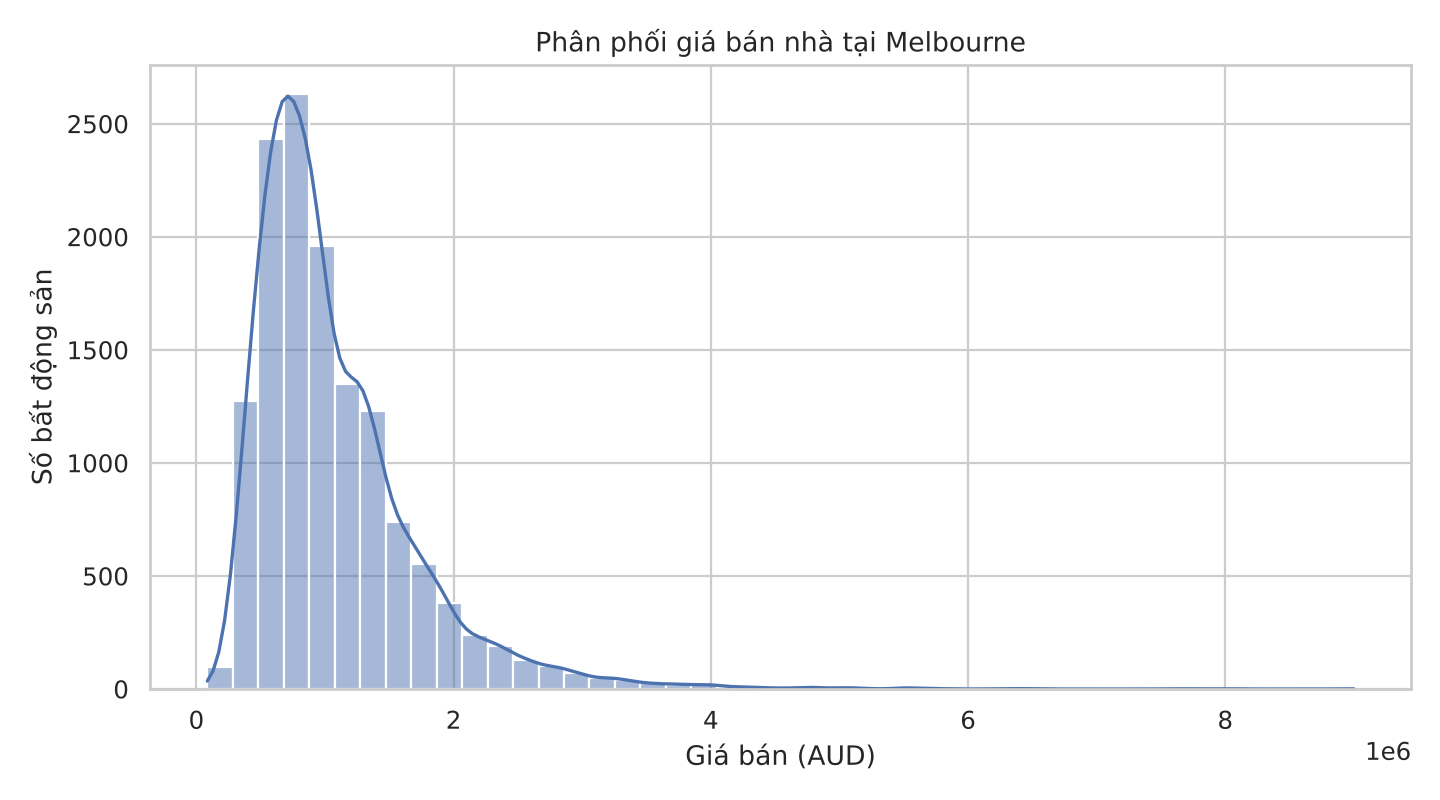
\includegraphics[width=0.72\linewidth]{01_price_distribution.png}
\caption{Phân phối giá bán nhà (histogram 45 khoảng kèm đường mật độ)}\label{fig:hist}
\nguon{\texttt{outputs/01\_price\_distribution.png}; số liệu kèm theo: \bs{P09}.}
\end{figure}

\paragraph{Diễn giải.} Trung bình cao hơn trung vị 19\% và đuôi phải kéo dài đến 9 triệu cho thấy phân phối lệch phải; 92.2\% giao dịch dưới 2 triệu (\bs{P09}). Vì vậy báo cáo dùng trung vị để so sánh nhóm, và logarit giá làm biến mục tiêu của Random Forest (mục~\ref{sec:ttr}). Trước khi loại ngoại lai, \texttt{Landsize} trung bình là 558.4 m\textsuperscript{2} (lớn nhất 433,014), sau khi loại là 478.3 trong khi trung vị gần như không đổi (440 và 439) (\bs{P02}).

\section{Giá theo nhóm (\texttt{groupby})}\label{sec:p2}\label{sec:p3}\label{sec:p4}\label{sec:p5}
Bốn phép dưới đây nhóm bằng \texttt{groupby}, lọc bằng \texttt{query} và sắp xếp bằng \texttt{sort\_values} trong \texttt{pipeline.py}.

\paragraph{Phép 2. Loại nhà.} Nhóm theo \texttt{Type}. Trung vị nhà riêng 1,080,000, liền kề 846,750, căn hộ 560,000, tức nhà riêng gấp 1.93 lần căn hộ và phân tán nhất (hệ số biến thiên 0.54 so với 0.42 và 0.43) (Bảng~\ref{tab:loainha}, Hình~\ref{fig:typebox}). Căn hộ nhỏ hơn (diện tích xây trung vị 75 m\textsuperscript{2} so với 144 m\textsuperscript{2}) và gần trung tâm hơn (6.9 km so với 10.4 km) (\bs{P03}), điều cần nhớ khi đọc tác động của khoảng cách ở Phép 6.

\begin{table}[H]
\centering
\caption{Giá theo loại nhà (AUD)}\label{tab:loainha}
\small
\begin{tabular}{@{}l r r r r r@{}}
\toprule
Loại nhà & Số giao dịch & Tỷ lệ & Trung vị & Trung bình & Hệ số biến thiên \\
\midrule
Nhà riêng (\texttt{h}) & 9,449 & 69.6\% & 1,080,000 & 1,242,665 & 0.54 \\
Liền kề (\texttt{t}) & 1,114 & 8.2\% & 846,750 & 933,735 & 0.42 \\
Căn hộ (\texttt{u}) & 3,017 & 22.2\% & 560,000 & 605,127 & 0.43 \\
\bottomrule
\end{tabular}
\nguon{\texttt{outputs/price\_by\_type.csv}; tỷ lệ: \bs{N09}; hệ số biến thiên: \bs{P03}.}
\end{table}

\begin{figure}[H]
\centering
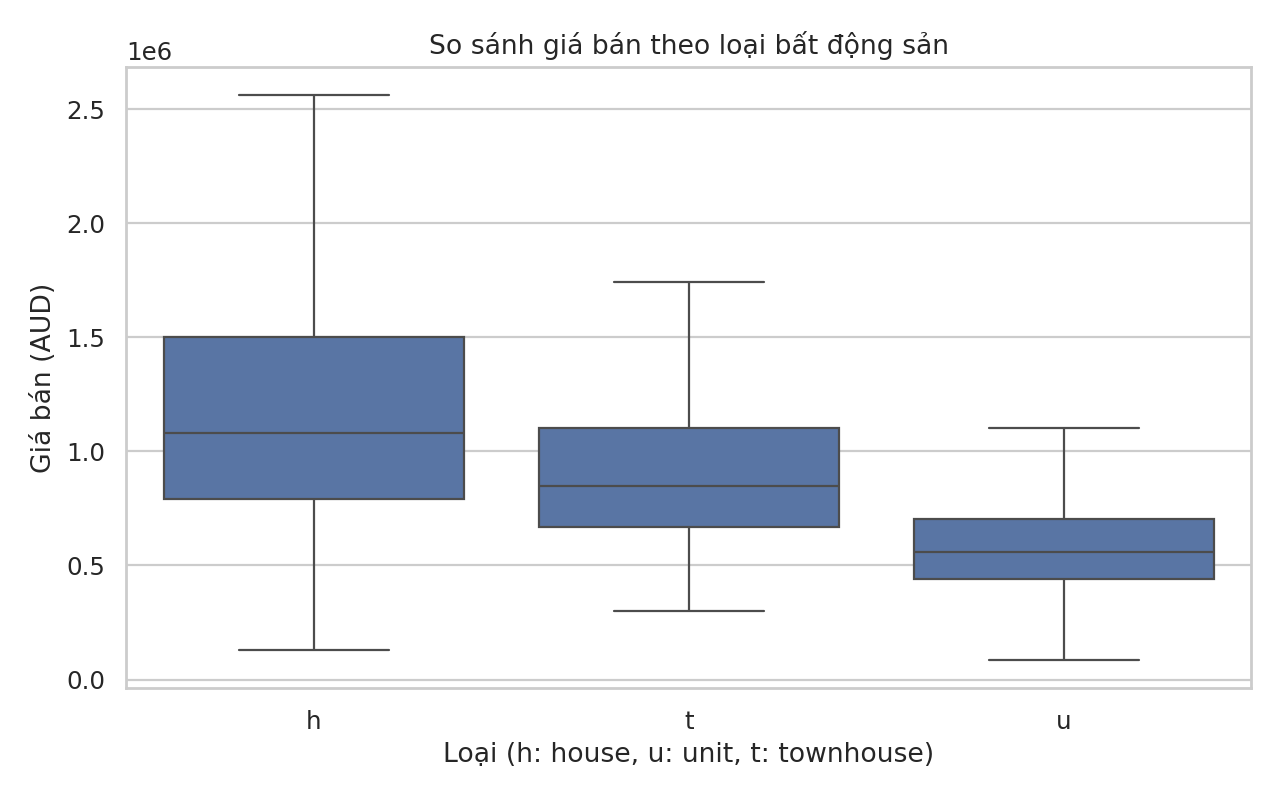
\includegraphics[width=0.72\linewidth]{02_price_by_type_boxplot.png}
\caption{Phân phối giá theo loại nhà (\texttt{h}: nhà riêng, \texttt{t}: liền kề, \texttt{u}: căn hộ)}\label{fig:typebox}
\nguon{\texttt{outputs/02\_price\_by\_type\_boxplot.png}; số liệu: \texttt{outputs/price\_by\_type.csv}.}
\end{figure}

\paragraph{Phép 3. Vùng.} Nhóm theo \texttt{Regionname} (8 vùng). Southern Metropolitan đắt nhất (trung vị 1,250,000), gấp 1.6 lần Western Metropolitan (793,000) (\bs{P04}; Hình~\ref{fig:region}). Ba vùng Victoria chỉ có 32 đến 53 giao dịch mỗi vùng nên kém tin cậy, và chênh lệch giữa các vùng còn lẫn với cơ cấu loại nhà.

\begin{figure}[H]
\centering
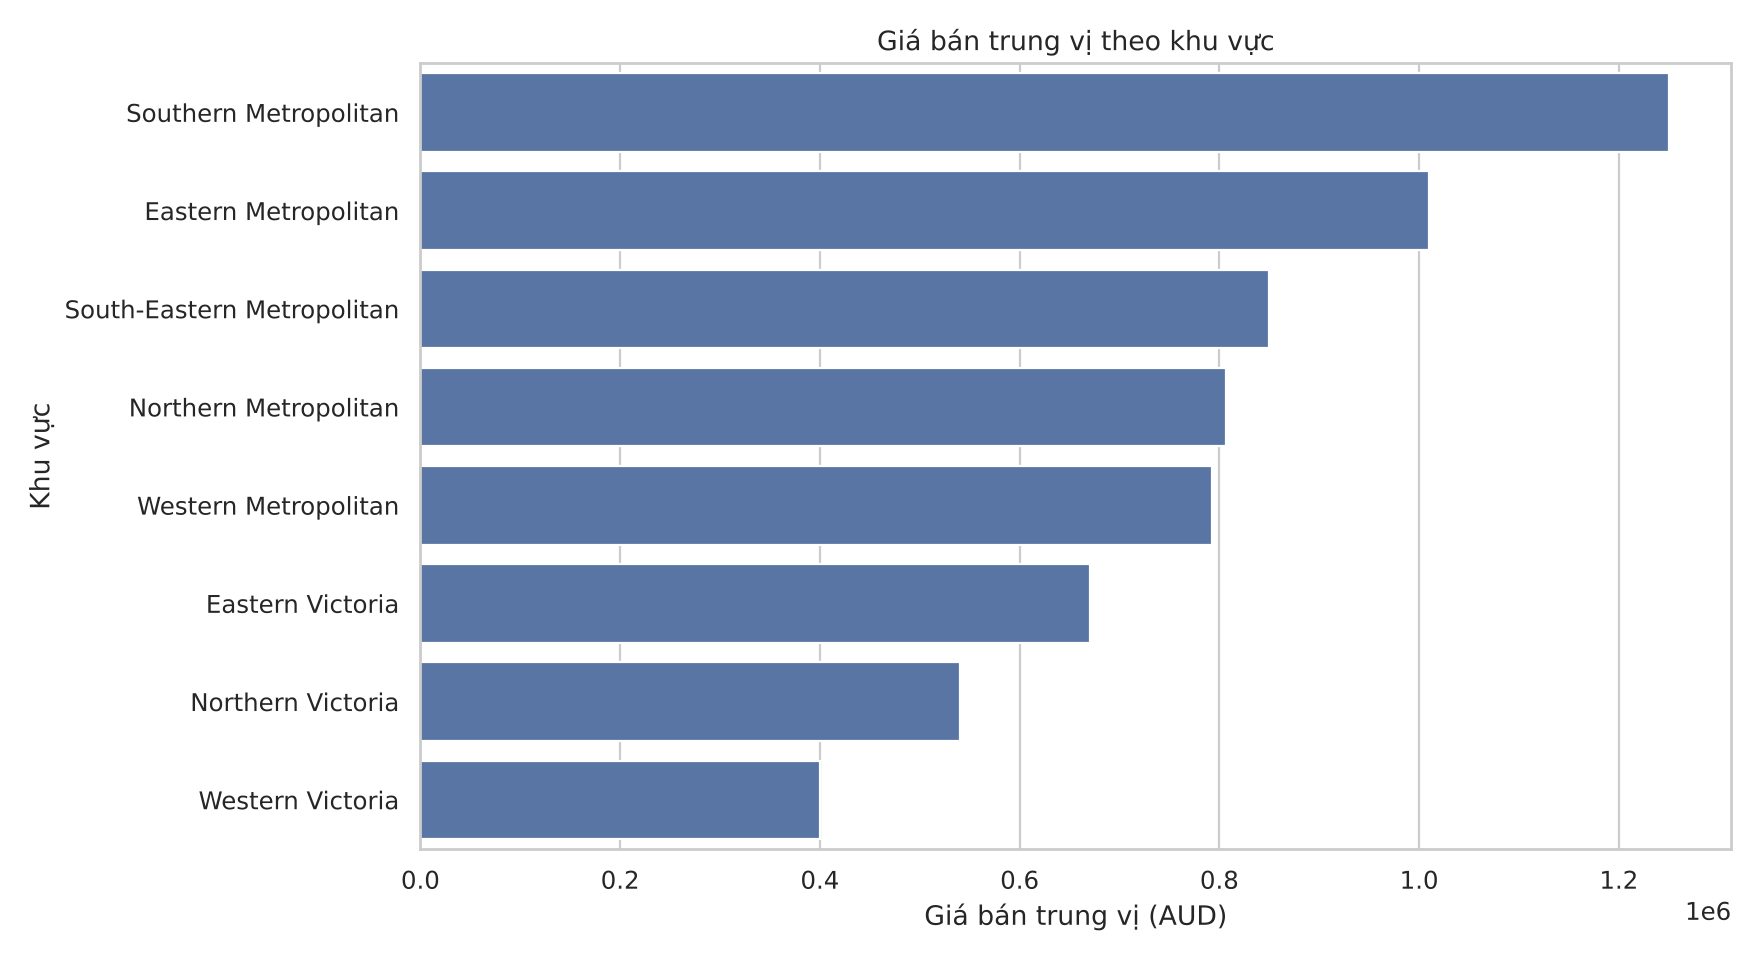
\includegraphics[width=0.72\linewidth]{03_median_price_by_region.png}
\caption{Giá trung vị theo vùng, sắp xếp giảm dần}\label{fig:region}
\nguon{\texttt{outputs/03\_median\_price\_by\_region.png}; số liệu: \texttt{outputs/price\_by\_region.csv}.}
\end{figure}

\paragraph{Phép 4. Số phòng.} Nhóm theo \texttt{Rooms}, giữ nhóm từ 20 giao dịch. Trung vị tăng từ 385,000 (1 phòng, 681 giao dịch) lên 690,000, 950,000, 1,285,000 và 1,660,000 (5 phòng); nhà 4 phòng đắt gấp 3.3 lần nhà 1 phòng, nhưng mức tăng thêm mỗi phòng giảm dần (+79\%, +38\%, +35\%, +29\%) (\bs{P05}; \texttt{outputs/price\_by\_rooms.csv}).

\paragraph{Phép 5. Suburb.} Nhóm theo \texttt{Suburb}, giữ suburb từ 30 giao dịch (125 trong 314 suburb; \bs{P06}) vì trung vị của suburb ít giao dịch dao động mạnh. Đứng đầu là Albert Park (1,900,000; 69 giao dịch), Canterbury (1,890,000), Middle Park (1,880,000), Balwyn (1,850,000) và Brighton (1,773,500), Albert Park gấp 2.1 lần trung vị chung (\texttt{outputs/top\_suburbs.csv}). Mô hình mã hóa suburb bằng one-hot (314 giá trị) nên các suburb thưa dữ liệu được học kém (mục~\ref{sec:hanche}).

\section{Tương quan với giá}\label{sec:tuongquan}\label{sec:p6}
\paragraph{Mục đích và phương pháp.} Xác định thuộc tính số liên hệ mạnh nhất với giá và kiểm tra ngoại lai về diện tích có làm sai lệch kết quả không: tính Pearson bằng \texttt{df[cols].corr()} và Spearman (\texttt{method="spearman"}), rồi so Pearson trước và sau khi loại ngoại lai (\texttt{build\_report\_metrics()}; ``trước khi loại'' là \texttt{data/melb\_data.csv} với \texttt{BuildingArea} $\leq$ 0 đặt thành thiếu).

\begin{figure}[H]
\centering
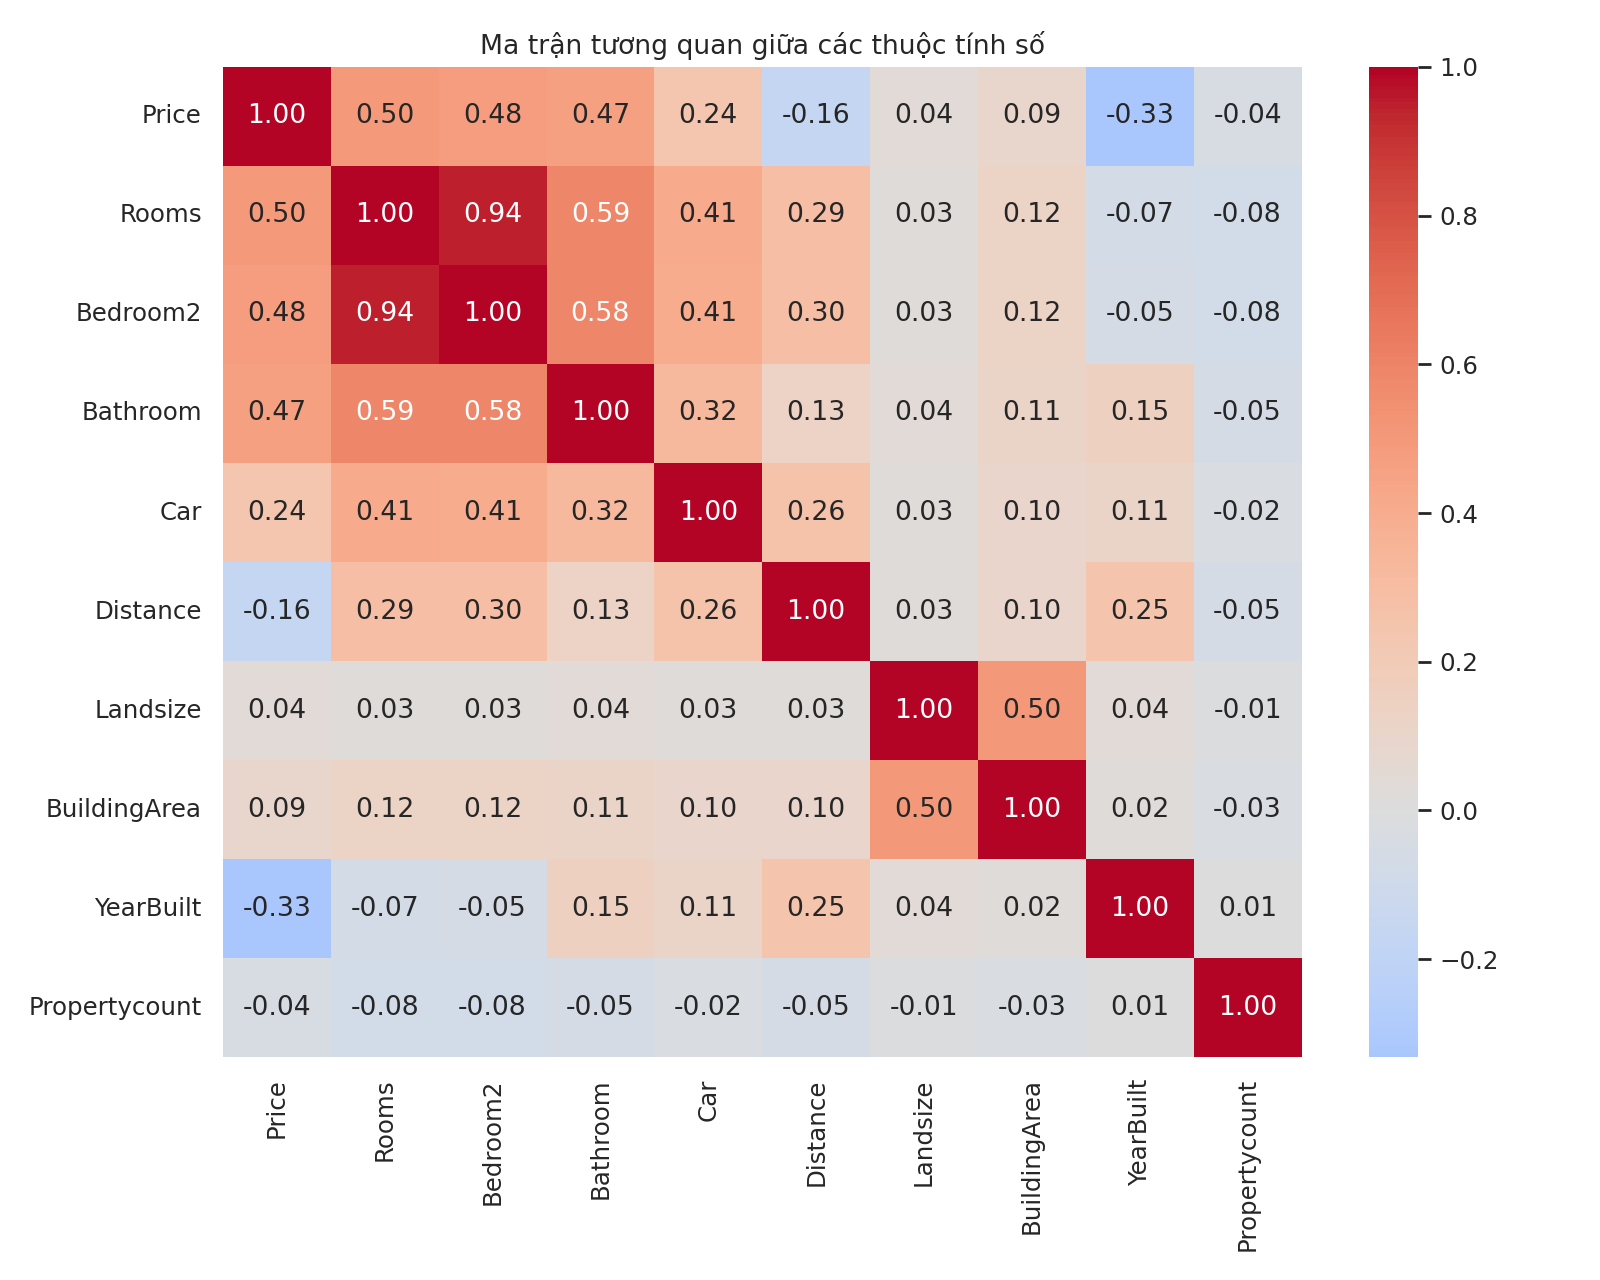
\includegraphics[width=0.8\linewidth]{05_correlation_heatmap.png}
\caption{Ma trận tương quan Pearson giữa giá và các thuộc tính số}\label{fig:corr}
\nguon{\texttt{outputs/05\_correlation\_heatmap.png}; giá trị: \bs{P07}.}
\end{figure}

\begin{table}[H]
\centering
\caption{Tương quan Pearson với giá trước và sau khi loại ngoại lai về diện tích}\label{tab:nhay}
\small
\begin{tabular}{@{}L{6.0cm} r r L{3.6cm}@{}}
\toprule
Thuộc tính & Trước & Sau & Spearman (sau) \\
\midrule
\texttt{BuildingArea} (loại 8 dòng $>$ 1,000 m\textsuperscript{2}) & 0.092 & 0.556 & 0.637 \\
\texttt{Landsize} (loại 26 dòng $>$ 10,000 m\textsuperscript{2}) & 0.038 & 0.132 & 0.329 \\
\bottomrule
\end{tabular}
\nguon{\bs{P07}; \texttt{outputs/price\_distance\_corr.csv} (một phần).}
\end{table}

\paragraph{Diễn giải.}
\begin{itemize}[nosep]
  \item Liên hệ mạnh nhất với giá: \texttt{BuildingArea} (0.556), \texttt{Rooms} (0.497), \texttt{Bedroom2} (0.476), \texttt{Bathroom} (0.469); \texttt{YearBuilt} ($-$0.332) và \texttt{Distance} ($-$0.163) tương quan âm. \texttt{Bedroom2} và \texttt{Rooms} gần như cùng một thông tin (0.944) (\bs{N06, P07}).
  \item Ngoại lai làm hệ số bị đánh giá thấp: tám dòng trên 1,000 m\textsuperscript{2} kéo Pearson của \texttt{BuildingArea} xuống 0.092; loại chúng thì hệ số lên 0.556, gần Spearman (0.637, không đổi vì dựa trên thứ hạng).
  \item \texttt{Distance} yếu khi gộp chung nhưng riêng nhà riêng là $-$0.329 và căn hộ gần như không phụ thuộc ($-$0.051) (\bs{P07}; Hình~\ref{fig:distance}). Giải thích khả dĩ là căn hộ rẻ hơn và gần trung tâm hơn; đây là giả thuyết chưa kiểm định. Pearson chỉ đo quan hệ tuyến tính, không chứng minh nhân quả.
\end{itemize}

\begin{figure}[H]
\centering
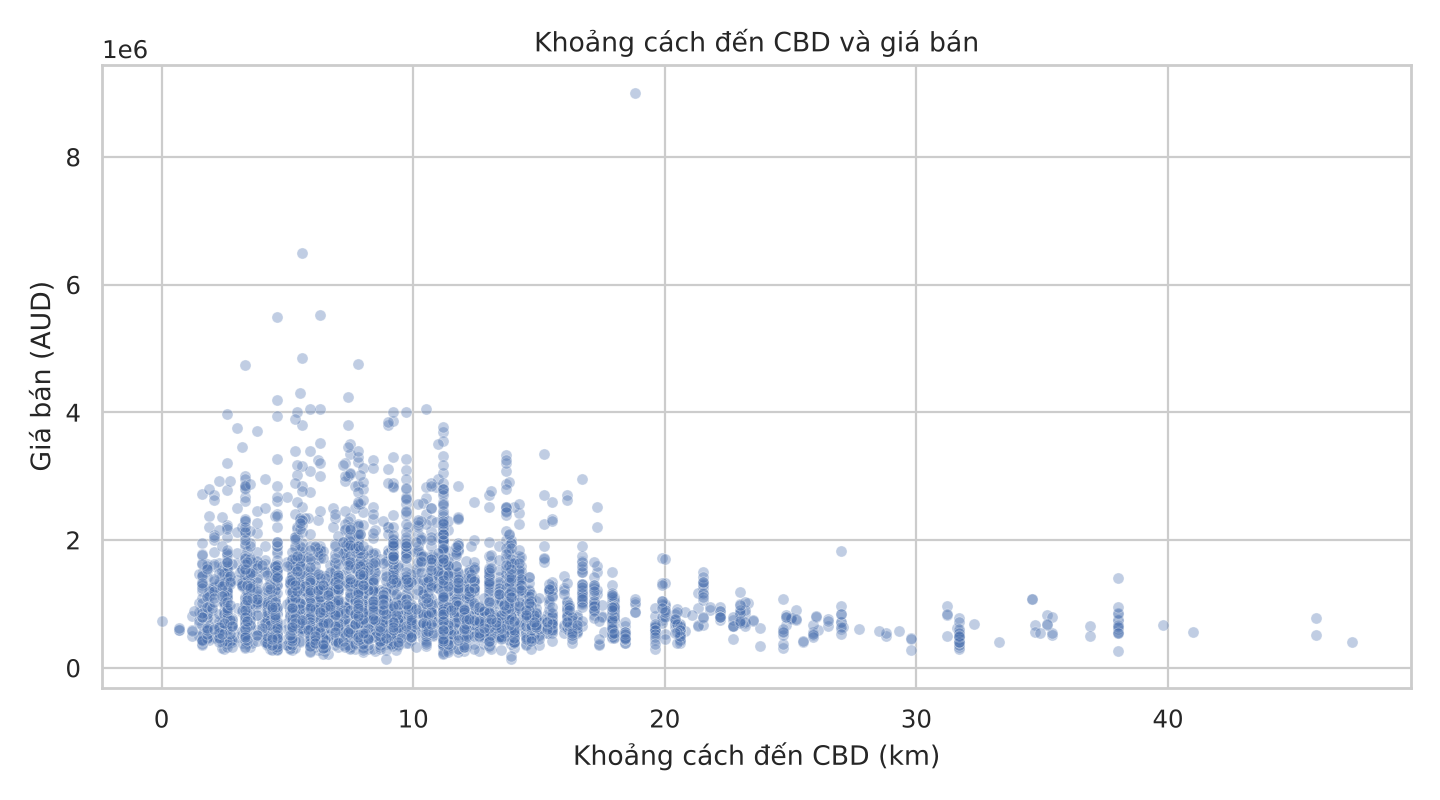
\includegraphics[width=0.72\linewidth]{04_price_vs_distance.png}
\caption{Khoảng cách đến trung tâm (CBD) và giá bán, mẫu ngẫu nhiên 4,000 điểm}\label{fig:distance}
\nguon{\texttt{outputs/04\_price\_vs\_distance.png}; hệ số tương quan: \bs{P07}; tỷ lệ theo khoảng cách: \bs{P09}.}
\end{figure}
Trong 1,007 giao dịch trên 2 triệu AUD, 97.2\% nằm trong 15 km; trong 731 giao dịch ngoài 20 km, 97.9\% dưới 1.5 triệu AUD (\bs{P09}).

\section{Theo thời gian}\label{sec:xuhuong}\label{sec:p7}
\paragraph{Phép 7. Giá theo tháng bán.} Nhóm theo \texttt{SaleMonth} và tính trung vị (\texttt{outputs/price\_by\_sale\_month.csv}). Trừ tháng 1 (2 giao dịch), trung vị dao động quanh 890,000 đến 970,000, trừ tháng 7 thấp rõ rệt (773,500) (\bs{P08}). Điểm trũng này cần đọc thận trọng: ở tháng 7/2017 chỉ 19.3\% giao dịch thuộc Southern Metropolitan (tháng 6: 29.5\%, tháng 8: 30.0\%), nên cơ cấu thiên về vùng rẻ hơn và giá thấp chưa chắc là giá giảm. Theo năm, trung vị gần như đi ngang: 900,000 (2016) và 910,000 (2017 đến 23/09), tăng khoảng 1.1\% (\bs{P08}). Dữ liệu chỉ dài 19 tháng và có khoảng trống nên kết luận chỉ có tính mô tả.

\chapter{Cơ sở lý thuyết scikit-learn}\label{ch:lythuyet}

Chương này giải thích các thành phần của scikit-learn mà \texttt{train\_model.py} sử dụng: vì sao được chọn, hoạt động thế nào và tham số nào đã đặt. Phần lý thuyết tổng quát lấy từ tài liệu scikit-learn \cite{sklearn-guide} và các công trình gốc \cite{pedregosa2011,hoerl1970,breiman2001}; phần gắn với đề tài dẫn tên hàm, biến trong mã nguồn và số liệu có mã truy nguồn. Bảng~\ref{tab:thanhphan} ở cuối chương tổng hợp toàn bộ thành phần.

\section{Giao diện thống nhất: estimator, transformer, predictor}\label{sec:api}
Mọi đối tượng trong scikit-learn tuân theo một số giao diện chung, nhờ đó các thành phần ghép được với nhau.
\begin{itemize}[nosep]
  \item \textbf{Estimator} là đối tượng học từ dữ liệu qua phương thức \texttt{fit(X, y)}. Những gì học được (trung vị, trung bình, hệ số, cây) lưu trong các thuộc tính kết thúc bằng dấu gạch dưới, ví dụ \texttt{coef\_}.
  \item \textbf{Transformer} biến đổi dữ liệu qua \texttt{transform(X)}; \texttt{fit\_transform} gộp hai bước. \texttt{SimpleImputer}, \texttt{StandardScaler} và \texttt{OneHotEncoder} là transformer.
  \item \textbf{Predictor} dự đoán qua \texttt{predict(X)}. \texttt{Ridge}, \texttt{RandomForest}\allowbreak\texttt{Regressor} và \texttt{DummyRegressor} là predictor.
\end{itemize}
Cần phân biệt \emph{tham số học được} (hệ số của Ridge, cấu trúc cây) với \emph{siêu tham số} do người dùng đặt trước khi học (\texttt{alpha}, \texttt{n\_estimators}). Nhờ cùng giao diện, vòng lặp so sánh mô hình trong \texttt{main()} của \texttt{train\_model.py} chỉ viết một lần: với mỗi mô hình trong từ điển \texttt{models}, gọi \texttt{fit} trên tập train, \texttt{predict} trên tập validation rồi đưa kết quả vào hàm \texttt{evaluate()}, áp dụng được cho cả Ridge và Random Forest.

\section{Rò rỉ dữ liệu, Pipeline và ColumnTransformer}\label{sec:pipeline}
\paragraph{Rò rỉ dữ liệu.} Nếu trung vị dùng để điền thiếu hoặc độ lệch chuẩn dùng để chuẩn hóa được tính trên \emph{toàn bộ} dữ liệu thì thông tin của tập validation và test lọt vào bước huấn luyện, làm sai số báo cáo lạc quan hơn thực tế. Quy tắc là mọi thống kê chỉ học từ tập train rồi áp dụng nguyên giá trị đó cho tập còn lại.

\paragraph{Pipeline.} \texttt{Pipeline} xếp các bước (transformer, rồi predictor ở cuối) thành một estimator duy nhất. Gọi \texttt{fit} trên pipeline là học từng bước trên dữ liệu được đưa vào; gọi \texttt{predict} áp dụng các tham số đã học. Vì pipeline được huấn luyện chỉ trên tập train (hoặc train gộp validation ở lần huấn luyện cuối), việc điền thiếu và chuẩn hóa tự động không rò rỉ. Ngoài ra pipeline đảm bảo lúc dự đoán dữ liệu mới đi qua đúng các bước đã dùng khi huấn luyện.

\paragraph{ColumnTransformer.} Cột số và cột phân loại cần xử lý khác nhau nên \texttt{ColumnTransformer} áp dụng từng pipeline con lên từng nhóm cột rồi ghép kết quả. Trong \texttt{build\_preprocessor()}, \texttt{remainder="drop"} loại các cột không khai báo (\texttt{Address}, \texttt{SellerG}, \texttt{Date}).

\begin{figure}[H]
\centering
\begin{tikzpicture}[node distance=7mm and 9mm, every node/.style={font=\small},
  box/.style={draw,rounded corners=2pt,align=center,minimum height=8mm,inner sep=4pt},
  arr/.style={-{Stealth[length=2mm]}}]
\node[box] (x) {Dữ liệu\\\footnotesize 23 đặc trưng};
\node[box,above right=2mm and 12mm of x] (n1) {Số: điền\\\footnotesize trung vị};
\node[box,right=of n1] (n2) {Số: chuẩn hóa\\\footnotesize \texttt{StandardScaler}};
\node[box,below right=2mm and 12mm of x] (c1) {Phân loại: điền\\\footnotesize giá trị phổ biến nhất};
\node[box,right=of c1] (c2) {Phân loại: one-hot\\\footnotesize \texttt{OneHotEncoder}};
\node[box,right=14mm of $(n2.east)!0.5!(c2.east)$] (m) {Mô hình\\\footnotesize Ridge / RF};
\draw[arr] (x.east) -- ++(4mm,0) |- (n1.west);
\draw[arr] (x.east) -- ++(4mm,0) |- (c1.west);
\draw[arr] (n1) -- (n2);
\draw[arr] (c1) -- (c2);
\draw[arr] (n2.east) -- ++(4mm,0) |- (m.west);
\draw[arr] (c2.east) -- ++(4mm,0) |- (m.west);
\end{tikzpicture}
\caption{Luồng xử lý trong \texttt{build\_preprocessor()} và mô hình (\texttt{Pipeline} bên ngoài, \texttt{ColumnTransformer} ở giữa)}\label{fig:luong}
\nguon{\texttt{train\_model.py}, hàm \texttt{build\_preprocessor()} và \texttt{build\_estimator()}.}
\end{figure}

\section{Các bộ tiền xử lý đã dùng}\label{sec:tienxuly}
\paragraph{SimpleImputer.} Thay ô thiếu bằng một thống kê học từ tập train. Đề tài dùng \texttt{strategy="median"} cho cột số và \texttt{"most\_frequent"} cho cột phân loại. Trung vị được chọn vì ít chịu ảnh hưởng của giá trị cực lớn hơn trung bình (xem Phép 1, Chương~\ref{ch:phantich}). Điền thiếu làm mất thông tin rằng ô vốn thiếu, nên các cột có thiếu đáng kể (\texttt{BuildingArea}, \texttt{YearBuilt}, \texttt{CouncilArea}, \texttt{Car}) được giữ thêm cờ \texttt{*\_was\_missing} từ bước làm sạch.

\paragraph{StandardScaler.} Biến đổi mỗi cột số thành
\[ z = \frac{x - \mu}{\sigma}, \]
với $\mu$, $\sigma$ là trung bình và độ lệch chuẩn của tập train. Bước này cần cho Ridge vì mức phạt $\alpha\lVert w\rVert^2$ (mục~\ref{sec:ridge}) phụ thuộc vào thang đo của cột: cột đo bằng mét vuông (hàng trăm) và cột số phòng (một chữ số) sẽ bị phạt không đồng đều nếu không chuẩn hóa. Với Random Forest, việc chuẩn hóa không làm đổi kết quả vì cây chỉ so sánh thứ tự giá trị; pipeline dùng chung nên vẫn chuẩn hóa.

\paragraph{OneHotEncoder.} Mỗi giá trị của biến phân loại thành một cột nhị phân (1 nếu dòng thuộc giá trị đó, 0 nếu không), tránh việc gán thứ tự giả cho các giá trị như tên suburb. Cái giá là số cột tăng theo số giá trị khác nhau: \texttt{Suburb} có 314 giá trị (\bs{P06}). Tham số \texttt{handle\_unknown="ignore"} làm giá trị chỉ xuất hiện ở tập test mã hóa thành toàn số 0 thay vì gây lỗi.

\section{Biến mục tiêu log: TransformedTargetRegressor}\label{sec:ttr}
Giá lệch phải (độ lệch 2.24; \bs{P01}), còn logarit giá gần đối xứng (độ lệch 0.18). \texttt{TransformedTargetRegressor} học trên $\log(1+y)$ (\texttt{func=np.log1p}) rồi đổi dự đoán về giá gốc bằng hàm ngược $\exp(\hat{u})-1$ (\texttt{inverse\_func=np.expm1}); mọi chỉ số vẫn tính bằng AUD. Học trên thang log làm sai số được đo theo tỷ lệ phần trăm hơn là theo số tuyệt đối, nên các căn giá thấp và giá cao được cân nhắc đồng đều hơn.

Có một lưu ý lý thuyết: nếu mô hình dự đoán tốt kỳ vọng của $\log(1+y)$ thì sau khi đổi ngược, kết quả gần với trung vị có điều kiện hơn là trung bình có điều kiện, vì $\exp$ là hàm lồi nên $\exp(\mathrm{E}[u]) \le \mathrm{E}[\exp(u)]$. Điều này có thể góp phần vào xu hướng dự đoán thấp ở nhóm giá cao (mục~\ref{sec:phankhuc}), nhưng báo cáo chưa kiểm chứng riêng nguyên nhân này.

\section{Ridge: hồi quy tuyến tính có phạt}\label{sec:ridge}
Hồi quy tuyến tính dự đoán $\hat{y} = w_0 + \sum_j w_j x_j$. Ridge chọn hệ số $w$ bằng cách cực tiểu hóa
\[ \sum_{i=1}^{n}\bigl(y_i - \hat{y}_i\bigr)^2 + \alpha \sum_{j} w_j^2 , \]
trong đó số hạng thứ hai (phạt L2) kéo các hệ số về gần 0; hệ số chặn $w_0$ không bị phạt \cite{hoerl1970}. $\alpha$ lớn thì mô hình đơn giản hơn (độ chệch tăng, phương sai giảm); $\alpha = 0$ trở về bình phương tối thiểu thông thường. Ridge hữu ích khi các đặc trưng tương quan với nhau, như \texttt{Rooms} và \texttt{Bedroom2} (tương quan 0.944; \bs{P07}), vì nghiệm bình phương tối thiểu khi đó không ổn định.

Đề tài dùng \texttt{Ridge(alpha=10.0, solver="lsqr")}. \texttt{lsqr} là bộ giải lặp, phù hợp khi ma trận đặc trưng có nhiều cột thưa do one-hot. Giá trị $\alpha = 10$ được đặt thủ công, không dò bằng cross-validation (mục~\ref{sec:quaykhop}). Giới hạn của mô hình là tuyến tính: nó không tự học tương tác (ví dụ ảnh hưởng của số phòng khác nhau giữa các suburb) hay quan hệ phi tuyến nếu không thêm đặc trưng tương ứng. Ridge học trên giá gốc (không qua log).

\section{Random Forest: tập hợp các cây quyết định}\label{sec:rf}
\paragraph{Cây quyết định hồi quy} chia không gian đặc trưng thành các vùng bằng chuỗi câu hỏi dạng ``\texttt{Rooms} $\le$ 3?'' và dự đoán trung bình giá của các dòng train rơi vào cùng một lá. Một cây đủ sâu khớp rất sát dữ liệu train nhưng dao động mạnh khi dữ liệu đổi (phương sai cao).

\paragraph{Random Forest} \cite{breiman2001} huấn luyện $B$ cây, mỗi cây trên một mẫu bootstrap (lấy mẫu có hoàn lại từ tập train), và ở mỗi lần chia chỉ xét một tập con ngẫu nhiên các đặc trưng. Dự đoán là trung bình của các cây:
\[ \hat{y}(x) = \frac{1}{B}\sum_{b=1}^{B} T_b(x). \]
Lấy trung bình nhiều cây ít tương quan làm giảm phương sai mà không tăng nhiều độ chệch. Ba siêu tham số đã đặt trong \texttt{train\_model.py}:
\begin{itemize}[nosep]
  \item \texttt{n\_estimators=100}: số cây $B$.
  \item \texttt{min\_samples\_leaf=2}: mỗi lá có ít nhất 2 dòng, hạn chế cây khớp từng dòng riêng lẻ.
  \item \texttt{max\_features=0.9}: mỗi lần chia xét 90\% số đặc trưng (số thực được hiểu là tỷ lệ).
\end{itemize}
Mô hình bắt được quan hệ phi tuyến và tương tác giữa các đặc trưng mà không cần khai báo. Hạn chế: mỗi dự đoán là trung bình của các giá trị giá có trong tập train nên không vượt ra ngoài khoảng giá đã thấy, và mô hình khó ngoại suy ở nhóm giá rất cao. Điều này phù hợp với quan sát giá dự đoán lớn nhất trên test là 4,246,907 trong khi giá thực lớn nhất là 6,500,000 (\bm{M02}); báo cáo không khẳng định đây là nguyên nhân duy nhất.

\section{Chia dữ liệu và vai trò của từng tập}\label{sec:chiatap}
\texttt{train\_test\_split} chia ngẫu nhiên có cố định hạt giống (\texttt{random\_state=42}) để kết quả tái lập được. Ba tập có ba vai trò:
\begin{itemize}[nosep]
  \item \textbf{Train}: học tham số của transformer và mô hình.
  \item \textbf{Validation}: so sánh các mô hình ứng viên và chọn một mô hình; có thể dùng nhiều lần.
  \item \textbf{Test}: đánh giá cuối cùng cho mô hình đã chọn, chỉ chấm một lần. Nếu dùng test để chọn mô hình thì sai số báo cáo bị lạc quan.
\end{itemize}
Mã chia hai lần với \texttt{test\_size=0.2}: lần một tách test 20\%, lần hai tách validation bằng 20\% phần còn lại, nên tỷ lệ thực là 64\% / 16\% / 20\% chứ không phải 60/20/20 (8,691 / 2,173 / 2,716 dòng; \bm{M06}). Sau khi chọn mô hình, \texttt{main()} huấn luyện lại trên train gộp validation (10,864 dòng) để tận dụng thêm dữ liệu; tập test không được dùng ở bước nào trước đó. Phép chia ngẫu nhiên chưa tính đến thứ tự thời gian của dữ liệu (mục~\ref{sec:hanche}).

\section{Các chỉ số đánh giá và baseline}\label{sec:chiso}
Gọi $y_i$ là giá thực, $\hat{y}_i$ là giá dự đoán, $n$ là số dòng đánh giá. \texttt{evaluate()} trong \texttt{train\_model.py} tính ba chỉ số đầu từ \texttt{sklearn.metrics}; MAPE do \texttt{build\_model\_error\_metrics()} tính trực tiếp từ \texttt{test\_predictions.csv}.
\begin{align*}
\mathrm{MAE} &= \frac{1}{n}\sum_i \lvert y_i-\hat{y}_i\rvert, &
\mathrm{RMSE} &= \sqrt{\frac{1}{n}\sum_i (y_i-\hat{y}_i)^2},\\
R^2 &= 1-\frac{\sum_i (y_i-\hat{y}_i)^2}{\sum_i (y_i-\bar{y})^2}, &
\mathrm{MAPE} &= \frac{1}{n}\sum_i \frac{\lvert y_i-\hat{y}_i\rvert}{y_i}.
\end{align*}
\begin{itemize}[nosep]
  \item MAE có đơn vị AUD, đọc trực tiếp được; chọn làm tiêu chí chọn mô hình.
  \item RMSE bình phương sai số nên phạt nặng dự đoán lệch lớn; RMSE lớn hơn MAE nhiều nghĩa là sai số tập trung ở một số ít dòng. Ở mô hình được chọn RMSE bằng 1.7 lần MAE (265,501 so với 156,203).
  \item $R^2$ so sai số của mô hình với sai số của việc luôn đoán $\bar{y}$ (trung bình của chính tập đang đánh giá). $R^2 = 1$ là hoàn hảo, $R^2 < 0$ là kém hơn dự đoán trung bình.
  \item MAPE đo sai số theo tỷ lệ phần trăm giá thực, giúp so sánh giữa các phân khúc giá khác nhau; nhược điểm là khuếch đại sai số ở căn giá thấp.
\end{itemize}

\paragraph{Baseline.} \texttt{DummyRegressor(strategy="median")} luôn dự đoán trung vị giá của tập train. Trong các hằng số, trung vị là giá trị làm MAE nhỏ nhất, nên đây là mốc MAE khó thua nhất mà không dùng thuộc tính nào. Baseline có $R^2$ âm ($-$0.0758) vì nó đoán trung vị của train, thấp hơn trung bình của tập test lệch phải (Chương~\ref{ch:mohinh}). Mô hình chỉ có giá trị nếu vượt rõ baseline.

\section{Quá khớp, dưới khớp và những gì báo cáo chưa kiểm tra}\label{sec:quaykhop}
\paragraph{Định nghĩa.} \emph{Quá khớp} (overfitting) là mô hình học cả nhiễu của tập train: sai số train rất thấp nhưng sai số trên dữ liệu chưa thấy cao hơn nhiều. \emph{Dưới khớp} (underfitting) là mô hình quá đơn giản: sai số cao ở cả train lẫn validation. Mô hình càng phức tạp thì độ chệch giảm và phương sai tăng (đánh đổi chệch--phương sai); mục tiêu là mức phức tạp mà sai số trên dữ liệu chưa thấy thấp nhất.

\paragraph{Cách kiểm tra.} So sai số train với sai số validation (khoảng cách lớn gợi ý quá khớp; cả hai cùng cao gợi ý dưới khớp), thay đổi siêu tham số rồi xem validation, hoặc vẽ đường cong học (\texttt{learning\_curve}). Siêu tham số có thể dò có hệ thống bằng \texttt{GridSearchCV} hoặc \texttt{RandomizedSearchCV} với cross-validation.

\paragraph{Tình trạng của đề tài.} Báo cáo \emph{chưa} tính sai số trên tập train nên không thể kết luận trực tiếp mô hình nào quá khớp hay dưới khớp. Hai quan sát gián tiếp: sai số test sát sai số validation (MAE 156,203 so với 154,865), nên bước chọn mô hình không gây lệch lớn; Ridge có MAE validation cao hơn Random Forest 49\% (231,160 so với 154,865), gợi ý một mô hình tuyến tính là quá đơn giản cho bài toán này, nhưng chỉ khi có sai số train của Ridge mới khẳng định được là dưới khớp. Random Forest vốn luôn có sai số train thấp hơn nhiều so với sai số trên dữ liệu mới, nên chênh lệch đó tự nó không phải bằng chứng xấu. Các siêu tham số hiện đặt thủ công, chưa dò (mục~\ref{sec:hanche}).

\section{Tổng hợp thành phần scikit-learn trong đề tài}\label{sec:tonghop}
\begin{table}[H]
\centering
\caption{Thành phần scikit-learn được dùng và vị trí trong \texttt{train\_model.py}}\label{tab:thanhphan}
\small
\begin{tabular}{@{}L{3.6cm} L{4.4cm} L{4.6cm}@{}}
\toprule
Thành phần & Vai trò & Tham số đã đặt \\
\midrule
\texttt{train\_test\_split} & Chia train, validation, test & \texttt{test\_size=0.2}, \texttt{random\_state=42}, gọi hai lần \\
\texttt{SimpleImputer} & Điền ô thiếu & \texttt{median} (số); \texttt{most\_frequent} (phân loại) \\
\texttt{StandardScaler} & Chuẩn hóa cột số & mặc định \\
\texttt{OneHotEncoder} & Mã hóa cột phân loại & \texttt{handle\_unknown="ignore"} \\
\texttt{ColumnTransformer} & Áp dụng xử lý riêng theo nhóm cột & \texttt{remainder="drop"} \\
\texttt{Pipeline} & Ghép tiền xử lý với mô hình & hai pipeline con và một pipeline ngoài \\
\texttt{Transformed}\allowbreak\texttt{TargetRegressor} & Học trên log giá, đổi ngược về AUD & \texttt{np.log1p}, \texttt{np.expm1} \\
\texttt{Ridge} & Hồi quy tuyến tính có phạt L2 & \texttt{alpha=10.0}, \texttt{solver="lsqr"} \\
\texttt{RandomForest}\allowbreak\texttt{Regressor} & Tập hợp các cây hồi quy & \texttt{n\_estimators=100}, \texttt{min\_samples\_leaf=2}, \texttt{max\_features=0.9}, \texttt{random\_state=42} \\
\texttt{DummyRegressor} & Baseline & \texttt{strategy="median"} \\
\texttt{mean\_absolute\_error}, \texttt{mean\_}\allowbreak\texttt{squared\_error}, \texttt{r2\_score} & MAE, RMSE, $R^2$ & trong \texttt{evaluate()} \\
\bottomrule
\end{tabular}
\nguon{\texttt{train\_model.py}, các hàm \texttt{build\_preprocessor}, \texttt{build\_estimator}, \texttt{evaluate} và \texttt{main}.}
\end{table}

\begin{thebibliography}{9}
\bibitem{sklearn-guide} scikit-learn developers. \emph{scikit-learn User Guide}. \url{https://scikit-learn.org/stable/user_guide.html}.
\bibitem{pedregosa2011} Pedregosa, F. và cs. Scikit-learn: Machine Learning in Python. \emph{Journal of Machine Learning Research}, 12, 2825--2830, 2011.
\bibitem{hoerl1970} Hoerl, A. E., Kennard, R. W. Ridge regression: biased estimation for nonorthogonal problems. \emph{Technometrics}, 12(1), 55--67, 1970.
\bibitem{breiman2001} Breiman, L. Random forests. \emph{Machine Learning}, 45(1), 5--32, 2001.
\end{thebibliography}

\chapter{Kết luận}\label{ch:ketluan}

\section{Các nhận xét chính từ dữ liệu}\label{sec:nhanxet}
Từ chín phép phân tích ở Chương~\ref{ch:phantich}, báo cáo rút ra bảy nhận xét. Mỗi nhận xét dẫn số liệu cụ thể và chỉ ra phép phân tích là nguồn của nó.
\begin{enumerate}
  \item \textbf{Loại nhà là yếu tố phân biệt giá mạnh nhất.} Giá trung vị của nhà riêng là 1,080,000 AUD, gấp 1.9 lần căn hộ (560,000); nhà liền kề ở giữa với 846,750 (Phép 2).
  \item \textbf{Vị trí tạo ra chênh lệch giá rất lớn, nhưng chủ yếu ở nhà riêng.} Suburb đắt nhất trong nhóm có từ 30 giao dịch (Albert Park, 1,900,000) gấp 3.9 lần suburb rẻ nhất (Werribee, 490,000). Giữa các vùng, nhà riêng ở Southern Metropolitan (1,650,000) gấp 1.9 lần ở Western Metropolitan (869,000), trong khi căn hộ chỉ chênh 1.3 lần (610,000 so với 460,000) (Phép 3, 7).
  \item \textbf{Khoảng cách đến trung tâm có ảnh hưởng, nhưng nếu chỉ nhìn số liệu gộp thì bị đánh giá thấp.} Tương quan giá--khoảng cách chung chỉ $-$0.163. Với nhà riêng nó gấp đôi ($-$0.329) và giá trung vị giảm 47\% từ 1,350,000 (trong 5 km) xuống 710,000 (trên 20 km), còn căn hộ gần như không đổi. Lý do là căn hộ rẻ nhưng tập trung ở gần trung tâm (42.7\% giao dịch trong 5 km đầu so với 5.3\% ở trên 20 km) (Phép 8).
  \item \textbf{Quy mô căn nhà có quan hệ đơn điệu rõ với giá.} Nhà 4 phòng có giá trung vị 1,285,000, gấp 3.3 lần nhà 1 phòng (385,000). Diện tích xây có Spearman 0.636 với giá, cao nhất trong các thuộc tính số, nhưng thuộc tính này thiếu 47.6\% giá trị (Phép 5, 8).
  \item \textbf{Giá lệch phải mạnh và phân khúc cao cấp khác hẳn phần còn lại.} Độ lệch của giá là 2.24 (0.18 sau khi lấy log); 18.7\% giao dịch từ 1,500,000 trở lên, trong đó 69\% ở Southern Metropolitan và 94.7\% là nhà riêng với diện tích xây trung vị 203 m\textsuperscript{2}, so với 76 m\textsuperscript{2} ở phân khúc dưới 600,000 (Phép 1, 9).
  \item \textbf{Trung vị thô theo thời gian che mất xu hướng.} Trung vị theo quý đi ngang trong khoảng 860,000--955,000, nhưng sau khi điều chỉnh cơ cấu suburb và loại nhà, giá tăng khoảng 10\% từ 2016Q2 (0.931) đến 2017Q1 (1.028) rồi ổn định quanh 1.02. Điểm trũng tháng 7/2017 (755,000) chủ yếu là hiệu ứng cơ cấu: chỉ số điều chỉnh của tháng đó vẫn là 1.001 (Phép 4, 6).
  \item \textbf{Dữ liệu thiếu mang thông tin.} Có 1,939 dòng có \texttt{Landsize} bằng 0, trong đó 1,629 dòng là căn hộ (54\% số căn hộ). Các dòng thiếu diện tích đất có giá trung vị 560,000, so với 973,250 ở các dòng có giá trị; nói cách khác ``thiếu'' ở đây gần như đồng nghĩa với ``căn hộ'' và không nên bị coi là nhiễu ngẫu nhiên (Chương~\ref{ch:lamsach}).
\end{enumerate}

\section{Hàm ý cho bước mô hình hóa}\label{sec:hamy}
Phần này chuyển các nhận xét trên thành quyết định cho mô hình dự đoán giá của dự án (chi tiết huấn luyện nằm ở \texttt{ml\_pipeline/PIPELINE.md}).

\subsection{Mục tiêu và đặc trưng nên dùng}
Bảng~\ref{tab:dactrung} liệt kê các nhóm đặc trưng giữ lại và bằng chứng từ phân tích.

\begin{table}[H]
\centering
\caption{Đặc trưng nên dùng và căn cứ từ phân tích dữ liệu}\label{tab:dactrung}
\small
\begin{tabular}{@{}L{3.6cm} L{3.6cm} L{6.6cm}@{}}
\toprule
Nhóm & Cách xử lý & Căn cứ \\
\midrule
Mục tiêu \texttt{Price} & Dự đoán log(giá), báo cáo lại bằng AUD & Độ lệch 2.24 giảm còn 0.18 (Phép 1) \\
\texttt{Type}, \texttt{Regionname} & One-hot & Ít giá trị (3 và 8) và phân biệt giá mạnh (Phép 2, 3); tương tác với nhau (Phép 7) \\
\texttt{Suburb}, \texttt{CouncilArea} & Target encoding, chỉ học trên train & Suburb có 314 giá trị, 59 suburb dưới 5 giao dịch; chênh giá 3.9 lần (Phép 3) \\
\texttt{Rooms}, \texttt{Bathroom}, \texttt{Car} & Số, điền thiếu bằng trung vị & Rooms 0.497, Bathroom 0.469 (Phép 5, 8) \\
\texttt{Distance}, \texttt{Lattitude}, \texttt{Longtitude} & Số & Distance có ảnh hưởng rõ khi tách loại nhà (Phép 8); tọa độ giúp mô hình học vị trí chi tiết \\
\texttt{Landsize}, \texttt{BuildingArea} & \texttt{log1p}, điền trung vị và thêm cờ ``đã thiếu'' & Lệch phải, có ngoại lai; thiếu mang thông tin (nhận xét 7) \\
\texttt{YearBuilt}, \texttt{HouseAge}, \texttt{SaleMonth} & Số, thêm cờ thiếu & Tuổi nhà tương quan 0.332 với giá, gián tiếp qua suburb và loại nhà (Phép 5); tháng bán cho mô hình bắt mức giá theo giai đoạn (Phép 6) \\
\bottomrule
\end{tabular}
\end{table}

\subsection{Các cột bị loại và cột nghi rò rỉ}
Rò rỉ (leakage) là việc mô hình dùng thông tin chỉ có sau khi giao dịch xảy ra hoặc thông tin gián tiếp chứa đáp án. Dự án chọn thời điểm dự đoán là \emph{lúc định giá}, nên chỉ dùng thuộc tính của căn nhà, vị trí và tháng bán.
\begin{itemize}[nosep]
  \item \texttt{Method} (phương thức bán) và \texttt{SellerG} (đại lý bán): chỉ biết khi quá trình bán đã diễn ra, và \texttt{Method} liên hệ với giá (trung vị phương thức \texttt{SP} là 770,000, thấp hơn \texttt{S} là 925,000). Đây là hai cột \emph{nghi rò rỉ} chính, bị loại.
  \item \texttt{Address}: gần như định danh (13,378 giá trị khác nhau trên 13,580 dòng), mô hình sẽ ghi nhớ thay vì khái quát.
  \item \texttt{Bedroom2}: trùng \texttt{Rooms} ở 95\% số dòng (tương quan 0.944), dư thừa.
  \item \texttt{Postcode}: trùng thông tin với suburb (198 mã so với 314 suburb).
  \item Các thống kê dùng để điền thiếu, chuẩn hóa và target encoding chỉ được học từ tập train; nếu học trên toàn bộ dữ liệu thì thông tin giá của tập kiểm tra sẽ rò vào mô hình qua suburb. Chỉ số điều chỉnh ở Phép 6 dùng trung vị trên toàn bộ dữ liệu nên \emph{chỉ để mô tả}, không được đưa vào mô hình.
\end{itemize}

\subsection{Phân khúc khó dự đoán và rủi ro dịch chuyển}
\begin{itemize}[nosep]
  \item \textbf{Nhà từ 1,500,000 trở lên} (18.7\% dữ liệu, tối đa 9,000,000): phân tán lớn (hệ số biến thiên của nhà riêng 0.54), ít mẫu ở đuôi và các giá trị cực đoan như căn 9,000,000 ở Mulgrave. Phân khúc này cần được theo dõi riêng khi đánh giá mô hình.
  \item \textbf{Phân khúc dưới 600,000} (19.6\%, 64.2\% là căn hộ): căn hộ có diện tích xây và đất thiếu nhiều, khoảng cách ít giải thích giá (Phép 8), nên khó dự đoán chính xác theo tỷ lệ.
  \item \textbf{Ba vùng Victoria ngoài đô thị} (32--53 giao dịch mỗi vùng) và các suburb thưa (59 suburb có dưới 5 dòng): kết quả không ổn định. Suburb chưa từng xuất hiện ở tập train phải được xử lý bằng giá trị mặc định của target encoding.
  \item \textbf{Dịch chuyển theo thời gian}: giá trung vị của ba tập là 910,000 (train), 816,000 (validation) và 1,001,000 (test),, tức mô hình huấn luyện trên giai đoạn cũ phải dự đoán ở mặt bằng giá khác. Đây là lý do dùng chia theo thời gian thay vì chia ngẫu nhiên: chia ngẫu nhiên sẽ che giấu rủi ro này và cho kết quả lạc quan.
\end{itemize}

\section{Hạn chế và hướng cải thiện}\label{sec:hanche}
Bảng~\ref{tab:hanche} nêu các hạn chế của dữ liệu và cách làm, cùng hướng cải thiện tương ứng.

\begin{table}[H]
\centering
\caption{Hạn chế và hướng cải thiện}\label{tab:hanche}
\small
\begin{tabular}{@{}L{7.0cm} L{6.7cm}@{}}
\toprule
Hạn chế & Hướng cải thiện \\
\midrule
Giai đoạn ngắn và có khoảng trống: 19 tháng có giao dịch, quý 1/2016 chỉ có 28 giao dịch, không có giao dịch tháng 3/2016 và tháng 1/2017. Không tách được mùa vụ khỏi xu hướng. & Thu thêm dữ liệu nhiều năm, đủ các tháng; khi đó mới ước lượng được mùa vụ và đánh giá mô hình qua nhiều chu kỳ giá. \\
Chỉ có các căn đã bán (thiên lệch chọn mẫu): không biết những căn không bán được. & Bổ sung dữ liệu niêm yết nếu có; nêu rõ phạm vi áp dụng của mô hình. \\
Giá danh nghĩa và không có biến vĩ mô (lãi suất, thu nhập, nguồn cung) nên không giải thích được diễn biến theo thời gian. & Thêm chuỗi vĩ mô theo tháng, hoặc quy đổi giá về một chỉ số giá nhà chung. \\
Dữ liệu thiếu nhiều: \texttt{BuildingArea} 47.6\%, \texttt{YearBuilt} 39.6\% (căn hộ gần như không có \texttt{Landsize}). & Thu thập thêm từ nguồn khác; điền thiếu theo suburb và loại nhà thay vì một trung vị chung (đã thêm cờ ``thiếu''). \\
Vùng và suburb thưa dữ liệu (ba vùng dưới 54 giao dịch; 59 suburb dưới 5 dòng). & Gộp nhóm nhỏ hoặc dùng mô hình phân cấp; target encoding hiện đã làm mịn một phần. \\
Vị trí chỉ có khoảng cách đến trung tâm và tọa độ, chưa có tiện ích (ga, trường học, công viên). & Thêm đặc trưng từ dữ liệu mở về giao thông và tiện ích. \\
Phân khúc cao cấp ít mẫu, sai số lớn; sai số hiện tại chưa đủ để định giá thay chuyên gia. & Dùng khoảng dự đoán hoặc hồi quy phân vị; đối chiếu với thẩm định thực tế. \\
Dữ liệu gốc được cào từ tin đăng công khai trên domain.com.au (Chương~\ref{ch:nguon}) nên có thể chứa sai lệch của tin đăng; đơn vị m\textsuperscript{2} của diện tích được suy ra chứ không có mô tả chính thức. & Đối chiếu thêm nguồn khác khi có thể; liên hệ tác giả bộ dữ liệu để xác nhận đơn vị. Chia sẻ lại dữ liệu phải theo CC BY-NC-SA 4.0 (ghi công, phi thương mại, chia sẻ tương tự). \\
\bottomrule
\end{tabular}
\end{table}

Ngoài ra, hàm thống kê theo khoảng cách (\texttt{stats\_by\_distance}) dùng khoảng mở ở cận dưới nên bỏ qua 6 dòng có khoảng cách bằng 0 (6 trên 13,580 dòng). Sai lệch nhỏ này đã được ghi chú ở Phép 8 và chưa được sửa trong mã.

\chapter{Kết luận}\label{ch:ketluan}

\section{Các nhận xét chính từ dữ liệu và mô hình}\label{sec:nhanxet}
Từ bảy phép phân tích ở Chương~\ref{ch:phantich} và kết quả mô hình ở Chương~\ref{ch:mohinh}, báo cáo rút ra chín nhận xét. Mỗi nhận xét dẫn số liệu cụ thể và chỉ ra nguồn của nó.
\begin{enumerate}
  \item \textbf{Loại nhà là yếu tố phân biệt giá mạnh.} Giá trung vị của nhà riêng là 1,080,000 AUD, gấp 1.93 lần căn hộ (560,000); nhà liền kề ở giữa với 846,750 (Phép 2).
  \item \textbf{Vị trí tạo ra chênh lệch giá lớn.} Southern Metropolitan có trung vị 1,250,000, cao hơn Western Metropolitan (793,000) khoảng 1.6 lần. Suburb đắt nhất trong nhóm có từ 30 giao dịch (Albert Park, 1,900,000) gấp 2.1 lần trung vị chung (903,000) (Phép 3, 5).
  \item \textbf{Số phòng có quan hệ đơn điệu rõ với giá.} Nhà 4 phòng có trung vị 1,285,000, gấp 3.3 lần nhà 1 phòng (385,000); Pearson giữa giá và số phòng là 0.497 (Phép 4, 6).
  \item \textbf{Khoảng cách đến trung tâm có ảnh hưởng, nhưng số liệu gộp đánh giá thấp nó.} Tương quan chung chỉ $-$0.163; riêng nhà riêng là $-$0.329, còn căn hộ gần như không phụ thuộc ($-$0.051), vì căn hộ rẻ nhưng tập trung gần trung tâm (Phép 6).
  \item \textbf{Giá lệch phải mạnh.} Độ lệch của giá là 2.24 và giảm còn 0.18 khi lấy log; trung bình (1,075,684) cao hơn trung vị (903,000) khoảng 19\% (Phép 1). Đây là lý do dùng trung vị khi so sánh và dùng log của giá khi huấn luyện Random Forest.
  \item \textbf{Ngoại lai diện tích che mờ tương quan.} Pearson của \texttt{BuildingArea} với giá là 0.092 khi còn dòng 44,515 m\textsuperscript{2}, nhưng 0.556 sau khi loại 8 dòng trên 1,000 m\textsuperscript{2}, gần Spearman (0.637); \texttt{Landsize} tăng từ 0.038 lên 0.132 sau khi loại 26 dòng trên 10,000 m\textsuperscript{2}. Diện tích xây là thuộc tính có tương quan cao nhất với giá (Phép 6).
  \item \textbf{Dữ liệu thiếu mang thông tin.} \texttt{BuildingArea} thiếu 47.7\% và \texttt{YearBuilt} thiếu 39.6\% sau làm sạch. Có 1,939 dòng \texttt{Landsize} bằng 0, trong đó 1,629 là căn hộ; các dòng này có giá trung vị 560,000 so với 975,000 ở các dòng có đất, và 84\% số dòng này là căn hộ (1,629 trên 1,939), nên giá trị 0 ở đây phản ánh loại nhà chứ không phải nhiễu ngẫu nhiên (Chương~\ref{ch:lamsach}).
  \item \textbf{Trung vị theo tháng chịu ảnh hưởng của cơ cấu giao dịch.} Tháng 7 có trung vị thấp nhất (773,500), nhưng riêng tháng 7/2017 chỉ có 19.3\% giao dịch ở Southern Metropolitan so với khoảng 30\% hai tháng kề bên, nên điểm trũng chưa chắc là giá giảm (Phép 7).
  \item \textbf{Mô hình vượt xa baseline nhưng yếu ở phân khúc cao cấp.} Random Forest đạt MAE 156,203 AUD trên tập test, thấp hơn baseline (439,350) 64.4\%, và $R^2$ là 0.8225. Với các căn từ 1,500,000 AUD, MAE tăng lên 368,100 và mô hình dự đoán thấp hơn thực tế trung bình 231,515 AUD (Chương~\ref{ch:mohinh}).
\end{enumerate}

\section{Hạn chế và hướng cải thiện}\label{sec:hanche}
Bảng~\ref{tab:hanche} nêu các hạn chế của dữ liệu và cách làm, cùng hướng cải thiện tương ứng. Những mục đầu là hạn chế của chính cách làm hiện tại và có thể sửa ngay.

\begin{table}[H]
\centering
\caption{Hạn chế và hướng cải thiện}\label{tab:hanche}
\small
\begin{tabular}{@{}L{7.0cm} L{6.7cm}@{}}
\toprule
Hạn chế & Hướng cải thiện \\
\midrule
Chia train/validation/test \emph{ngẫu nhiên} trong khi dữ liệu có ngày bán; sai số có thể lạc quan so với dự báo giai đoạn sau. & Chia theo thời gian (train là các tháng đầu, test là các tháng cuối) và báo cáo cả hai cách để thấy chênh lệch. \\
Mô hình dùng \texttt{Method} (chỉ biết sau khi bán), \texttt{Postcode} (trùng thông tin suburb) và \texttt{Bedroom2} (trùng \texttt{Rooms} 95\%). & Chạy lại không có \texttt{Method} (và thử bỏ thêm \texttt{Postcode}, \texttt{Bedroom2}) để đo sai số thật khi định giá trước lúc bán; giữ phiên bản nào tùy mục tiêu. \\
Siêu tham số của Ridge và Random Forest đặt cố định, chưa tinh chỉnh; mới có hai mô hình ứng viên. & Tìm siêu tham số bằng kiểm định chéo trên tập train; thử thêm mô hình tăng cường gradient (ví dụ \texttt{HistGradientBoostingRegressor}, xử lý được giá trị thiếu). \\
Phân khúc từ 1,500,000 AUD có sai số lớn và bị dự đoán thấp (lệch $+$231,515). & Dùng hồi quy phân vị hoặc khoảng dự đoán, hoặc mô hình riêng cho phân khúc cao cấp; báo cáo thêm MAPE theo phân khúc. \\
Suburb có 314 giá trị, 59 suburb dưới 5 giao dịch; one-hot cho các suburb thưa học kém. & Gộp các suburb thưa hoặc dùng mã hóa mục tiêu có làm mịn (chỉ \texttt{fit} trên tập train). \\
Giai đoạn ngắn và có khoảng trống: 19 tháng có giao dịch, quý 1/2016 chỉ có 28 giao dịch, không có giao dịch tháng 3/2016 và tháng 1/2017; không tách được mùa vụ khỏi xu hướng. & Thu thêm dữ liệu nhiều năm, đủ các tháng. \\
Chỉ có các căn đã bán (thiên lệch chọn mẫu) và giá danh nghĩa, không có biến vĩ mô (lãi suất, thu nhập, nguồn cung). & Bổ sung dữ liệu niêm yết và chuỗi vĩ mô theo tháng nếu có; nêu rõ phạm vi áp dụng của mô hình. \\
Vị trí chỉ có khoảng cách đến trung tâm và tọa độ, chưa có tiện ích (ga, trường học, công viên). & Thêm đặc trưng từ dữ liệu mở về giao thông và tiện ích. \\
Dữ liệu gốc được cào từ tin đăng công khai trên domain.com.au (Chương~\ref{ch:nguon}) nên có thể chứa sai lệch của tin đăng; đơn vị m\textsuperscript{2} của diện tích được suy ra chứ không có mô tả chính thức. & Đối chiếu thêm nguồn khác khi có thể; liên hệ tác giả bộ dữ liệu để xác nhận đơn vị. Chia sẻ lại dữ liệu phải theo CC BY-NC-SA 4.0 (ghi công, phi thương mại, chia sẻ tương tự). \\
\bottomrule
\end{tabular}
\end{table}


\begin{thebibliography}{9}
\addcontentsline{toc}{chapter}{Tài liệu tham khảo}
\bibitem{melbourne-kaggle} Pino, T. (dansbecker). \emph{Melbourne Housing Snapshot}. Kaggle, CC BY-NC-SA 4.0. \url{https://www.kaggle.com/datasets/dansbecker/melbourne-housing-snapshot}.
\bibitem{sklearn-guide} scikit-learn developers. \emph{scikit-learn User Guide}. \url{https://scikit-learn.org/stable/user_guide.html}.
\bibitem{pedregosa2011} Pedregosa, F. và cs. Scikit-learn: Machine Learning in Python. \emph{Journal of Machine Learning Research}, 12, 2825--2830, 2011.
\bibitem{buitinck2013} Buitinck, L. và cs. API design for machine learning software: experiences from the scikit-learn project. \emph{ECML PKDD Workshop: Languages for Data Mining and Machine Learning}, 108--122, 2013. arXiv:1309.0238.
\bibitem{hoerl1970} Hoerl, A. E., Kennard, R. W. Ridge regression: biased estimation for nonorthogonal problems. \emph{Technometrics}, 12(1), 55--67, 1970.
\bibitem{breiman2001} Breiman, L. Random forests. \emph{Machine Learning}, 45(1), 5--32, 2001.
\end{thebibliography}

\appendix
\addtocontents{toc}{\protect\renewcommand{\protect\cftchappresnum}{Phụ lục }}
\chapter{Bảng đầy đủ quy tắc làm sạch}\label{pl:quytac}

\section*{A.1. Bảy quy tắc và đoạn mã tương ứng}
Mã nguồn dưới đây là hàm \texttt{clean()} trong \texttt{ml\_pipeline/features.py}. Các quy tắc không dùng thống kê của tập dữ liệu nào, nên áp dụng giống hệt cho dữ liệu huấn luyện và dữ liệu nhập từ giao diện.

\begin{table}[H]
\centering
\caption{Quy tắc làm sạch, câu lệnh, lý do và số dòng bị ảnh hưởng}\label{tab:quytac-day-du}
\small
\setlength{\tabcolsep}{4pt}
\begin{tabular}{@{}c L{4.6cm} L{4.8cm} L{2.7cm} r@{}}
\toprule
\# & Câu lệnh & Lý do & Hành động & Số dòng \\
\midrule
1 & \texttt{YearBuilt < 1800} & Năm nhỏ nhất là 1196, không thể có & Đặt thành thiếu & 1 \\
2 & \texttt{Landsize == 0} & Đất 0 m\textsuperscript{2} nghĩa là không có số liệu, nhất là căn hộ (1,629 trong 1,939 dòng) & Đặt thành thiếu & 1,939 \\
3 & \texttt{Landsize > 100000} & 433,014 m\textsuperscript{2} phi thực tế cho một căn nhà & Đặt thành thiếu & 1 \\
4 & \texttt{BuildingArea == 0} & Diện tích xây bằng 0 không hợp lý & Đặt thành thiếu & 17 \\
5 & \texttt{BuildingArea > 10000} & 44,515 m\textsuperscript{2}, ngoại lai phi thực tế & Đặt thành thiếu & 1 \\
6 & \texttt{Bathroom == 0} & Nhà ở bán không thể không có phòng tắm & Đặt thành thiếu & 34 \\
7 & \texttt{CouncilArea} thiếu & Giữ ``không biết'' thành một nhóm riêng thay vì bỏ dòng & Điền ``Unknown'' & 1,369 \\
\midrule
 & \multicolumn{2}{l}{Tổng số dòng bị xóa} & & 0 \\
\bottomrule
\end{tabular}
\end{table}

\begin{lstlisting}
def clean(df):
    d = df.copy()
    d["Date"] = pd.to_datetime(d["Date"], format="%d/%m/%Y", errors="coerce")
    d.loc[d["YearBuilt"] < 1800, "YearBuilt"] = np.nan  # 1
    d.loc[d["Landsize"] == 0, "Landsize"] = np.nan  # 2
    d.loc[d["Landsize"] > 100_000, "Landsize"] = np.nan  # 3
    d.loc[d["BuildingArea"] == 0, "BuildingArea"] = np.nan  # 4
    d.loc[d["BuildingArea"] > 10_000, "BuildingArea"] = np.nan  # 5
    d.loc[d["Bathroom"] == 0, "Bathroom"] = np.nan  # 6
    d["CouncilArea"] = d["CouncilArea"].fillna("Unknown")  # 7
    return d
\end{lstlisting}
Số ở cuối mỗi dòng chú thích khớp với cột \# của Bảng~\ref{tab:quytac-day-du}. Dòng đầu tiên chỉ đổi cột \texttt{Date} từ chuỗi sang kiểu ngày khi cột này còn là chuỗi.

\section*{A.2. Số ô thiếu trước và sau làm sạch}
Làm sạch chuyển giá trị không hợp lệ thành thiếu nên số ô thiếu thay đổi như Bảng~\ref{tab:thieu-truoc-sau}. Cột \texttt{HouseAge} là biến dẫn xuất (năm bán trừ \texttt{YearBuilt}) nên không có trong tệp gốc.

\begin{table}[H]
\centering
\caption{Số ô thiếu trước và sau làm sạch (13,580 dòng)}\label{tab:thieu-truoc-sau}
\small
\begin{tabular}{@{}l r r r@{}}
\toprule
Cột & Trước & Sau & Thay đổi \\
\midrule
\texttt{Landsize} & 0 & 1,940 & +1,940 (quy tắc 2 và 3) \\
\texttt{BuildingArea} & 6,450 & 6,468 & +18 (quy tắc 4 và 5) \\
\texttt{YearBuilt} & 5,375 & 5,376 & +1 (quy tắc 1) \\
\texttt{Bathroom} & 0 & 34 & +34 (quy tắc 6) \\
\texttt{Car} & 62 & 62 & không đổi \\
\texttt{CouncilArea} & 1,369 & 0 & $-$1,369 (quy tắc 7) \\
\texttt{HouseAge} (dẫn xuất) & --- & 5,382 & 5,376 từ \texttt{YearBuilt} thiếu, thêm 6 dòng tuổi nhà âm \\
\bottomrule
\end{tabular}
\end{table}

\section*{A.3. Biến dẫn xuất và cột bị loại}
Hàm \texttt{engineer()} thêm hai biến chỉ dựa trên chính dòng đó (không dùng thống kê của tập nào):
\begin{itemize}[nosep]
  \item \texttt{SaleMonth}: tháng bán, lấy từ cột \texttt{Date};
  \item \texttt{HouseAge}: năm bán trừ \texttt{YearBuilt}; giá trị âm (6 dòng có năm xây sau ngày bán) được đặt thành thiếu.
\end{itemize}
Năm cột bị loại khỏi mô hình (\texttt{DROP\_COLS}): \texttt{Address} (gần như định danh), \texttt{Bedroom2} (trùng \texttt{Rooms} ở 95\% số dòng), \texttt{Method} và \texttt{SellerG} (chỉ biết sau khi bán, nghi rò rỉ) và \texttt{Postcode} (trùng thông tin suburb). Lý do chi tiết ở mục~\ref{sec:hamy}. Các cột này vẫn được giữ trong dữ liệu để phân tích và hiển thị; chỉ không đưa vào mô hình.


\chapter{Ánh xạ tiêu chí nghiệm thu mục 1 đến 3 với vị trí trong báo cáo}\label{pl:anhxa}

Bảng~\ref{tab:anhxa} đối chiếu từng tiêu chí đạt ở mục 1 đến 3 của \texttt{docs/01\_QuyTac\_YeuCau.md} với nơi tiêu chí được đáp ứng trong báo cáo, để kiểm tra trước khi nộp. Cột trạng thái nêu thẳng các điểm còn thiếu.

\begin{longtable}{@{}L{0.9cm} L{5.2cm} L{3.6cm} L{4.2cm}@{}}
\caption{Đối chiếu tiêu chí nghiệm thu với vị trí trong báo cáo}\label{tab:anhxa}\\
\toprule
Mục & Tiêu chí đạt (rút gọn) & Vị trí trong báo cáo & Trạng thái \\
\midrule
\endfirsthead
\toprule
Mục & Tiêu chí đạt (rút gọn) & Vị trí trong báo cáo & Trạng thái \\
\midrule
\endhead
\midrule
\multicolumn{4}{r}{\emph{Còn tiếp ở trang sau}}\\
\endfoot
\bottomrule
\endlastfoot
\multicolumn{4}{@{}l}{\textbf{Mục 1. Dữ liệu}} \\
1.1 & Mục ``Nguồn dữ liệu'': tên, nơi lấy, giấy phép, cách thu thập, số bản ghi và thuộc tính, ý nghĩa cột chính & Mục~\ref{sec:nguon} (Bảng~\ref{tab:nguon}), mục~\ref{sec:quymo} (Bảng~\ref{tab:quymo}), mục~\ref{sec:tudien} (Bảng~\ref{tab:tudien}) & Đạt: tên, nơi lấy, giấy phép (CC BY-NC-SA 4.0), cách thu thập gốc (web scraping qua domain.com.au), quy mô, ý nghĩa cột \\
1.2 & Dữ liệu thô giữ nguyên trong \texttt{data/}, mọi biến đổi qua mã & Mục~\ref{sec:nguyenven} & Đạt \\
1.3 & Tối thiểu khoảng 500 bản ghi và 5 thuộc tính & Mục~\ref{sec:quymo} (13,580 bản ghi, 21 thuộc tính) & Đạt \\
\midrule
\multicolumn{4}{@{}l}{\textbf{Mục 2. Xử lý dữ liệu}} \\
2.1 & Kiểm tra kiểu dữ liệu, dữ liệu thiếu, trùng lặp, giá trị lỗi, kèm số liệu & Mục~\ref{sec:kiemtra} (Bảng~\ref{tab:kiemtra}, \ref{tab:loi}) & Đạt \\
2.2 & Mỗi quy tắc làm sạch ghi số dòng bị ảnh hưởng; không xóa dòng khi chưa nêu lý do & Mục~\ref{sec:quytac} (Bảng~\ref{tab:quytac}), Phụ lục~\ref{pl:quytac} & Đạt (0 dòng bị xóa) \\
2.3 & Dùng \texttt{groupby}, lọc, sắp xếp hoặc tổng hợp & Mục~\ref{sec:groupby}, Phép 3 (lọc suburb từ 30 giao dịch rồi sắp xếp), Phép 7, 9 & Đạt \\
2.4 & Tiền xử lý dùng chung giữa huấn luyện và giao diện, một nguồn \texttt{features.py} & Mục~\ref{sec:dungchung} (Hình~\ref{fig:dungchung}) & Đạt \\
2.5 & Thống kê điền, chuẩn hóa, mã hóa chỉ học từ tập train & Mục~\ref{sec:thieu}, mục~\ref{sec:chia} & Đạt \\
\midrule
\multicolumn{4}{@{}l}{\textbf{Mục 3. Phân tích và trực quan hóa}} \\
3.1 & Ít nhất 5 phép phân tích, mỗi phép có mục đích, phương pháp, kết quả, diễn giải & Chương~\ref{ch:phantich} (9 phép) & Đạt \\
3.2 & Ít nhất 4 biểu đồ thuộc ít nhất 3 dạng & Mục~\ref{sec:bieudo} (7 biểu đồ, 6 dạng) & Đạt \\
3.3 & Ít nhất 3 nhận xét có ý nghĩa, mỗi nhận xét dẫn số liệu & Mục~\ref{sec:nhanxet} (7 nhận xét) & Đạt \\
3.4 & Biểu đồ có tiêu đề, nhãn trục, đơn vị & Mục~\ref{sec:nguyentac}, \ref{sec:bieudo} & Đạt; ở heatmap hai trục là tên thuộc tính nên không có đơn vị \\
3.5 & Phần phân tích hiển thị được trong ứng dụng & Mục~\ref{sec:streamlit} (tab Phân tích dữ liệu) & Chức năng đạt. Còn thiếu: hai ảnh chụp màn hình thật (Hình~\ref{fig:app-tongquan}, \ref{fig:app-bieudo} đang là khung giữ chỗ) \\
3.6 & Notebook theo luồng Dataset $\to$ Data Cleaning $\to$ Analysis $\to$ Visualization $\to$ Conclusions & Notebook phân tích trong \texttt{ml\_pipeline/} (mục 1--7); báo cáo theo cùng thứ tự: Chương~\ref{ch:nguon} đến~\ref{ch:ketluan} & Đạt; notebook có thêm mục mô hình trước phần kết luận \\
\end{longtable}

Trước khi nộp bài, cần bổ sung thông tin bìa (trường, khoa, họ tên, mã số sinh viên, giảng viên hướng dẫn trong \texttt{main.tex}) và hai ảnh chụp màn hình.


\chapter{Hướng dẫn tái lập kết quả}\label{pl:taile}

Các lệnh dưới đây bắt đầu từ thư mục gốc của kho mã (repo) và ghi rõ khi cần chuyển thư mục. Dữ liệu thô nằm ở \texttt{data/melb\_data.csv}; không cần tải thêm gì.

\section*{C.1. Cài đặt}
Cần Python 3 và các thư viện trong \texttt{requirements.txt}:
\begin{lstlisting}[language=bash]
cd ml_pipeline
pip install -r requirements.txt
\end{lstlisting}

\section*{C.2. Chạy notebook phân tích}
Notebook là \texttt{ml\_pipeline/Housing\_Price\_Analysis.ipynb}. Gói Jupyter không nằm trong \texttt{requirements.txt} nên cài thêm. Notebook đọc dữ liệu bằng đường dẫn tương đối \texttt{../data/melb\_data.csv}, vì vậy phải mở từ thư mục \texttt{ml\_pipeline}:
\begin{lstlisting}[language=bash]
pip install notebook
cd ml_pipeline
jupyter notebook Housing_Price_Analysis.ipynb
\end{lstlisting}
Trong Jupyter chọn \emph{Run All} để chạy toàn bộ các ô. Hai bước đầu của notebook cũng có dạng chương trình riêng trong \texttt{ml\_pipeline/}: \texttt{01\_eda.py} (kiểm tra và khám phá dữ liệu) và \texttt{02\_prep.py} (làm sạch, chia theo thời gian, tiền xử lý), chạy bằng \texttt{python} như một tệp thông thường.

\section*{C.3. Chạy ứng dụng (tùy chọn)}
Tab \emph{Phân tích dữ liệu} của ứng dụng hiển thị lại các kết quả của báo cáo và dùng được ngay, không cần đăng nhập hay cơ sở dữ liệu:
\begin{lstlisting}[language=bash]
cd ml_pipeline
streamlit run app.py
\end{lstlisting}
Phần đăng nhập, cơ sở dữ liệu và triển khai bằng Docker không thuộc phạm vi báo cáo này; cách chạy xem trong \texttt{README.md}.

\section*{C.4. Chạy kiểm thử}
\begin{lstlisting}[language=bash]
cd ml_pipeline
python -m pytest -q
\end{lstlisting}

\section*{C.5. Biên dịch báo cáo}
Cần bản TeX có \texttt{xelatex} cùng gói \texttt{polyglossia} (tiếng Việt) và phông TeX Gyre (Termes, Heros, Cursor); trên Overleaf chọn trình biên dịch XeLaTeX. Hình được sinh lại từ dữ liệu thật bằng \texttt{make\_figures.py}, sau đó biên dịch hai lần để mục lục, danh mục hình và danh mục bảng cập nhật đúng (thỉnh thoảng cần lần thứ ba):
\begin{lstlisting}[language=bash]
cd report
python make_figures.py
xelatex main.tex
xelatex main.tex
\end{lstlisting}
Để chèn ảnh chụp màn hình thật, lưu hai tệp \texttt{tab-phan-tich-tong-quan.png} và \texttt{tab-phan-tich-bieu-do.png} vào \texttt{report/screenshots/} rồi biên dịch lại; thông tin bìa sửa ở đầu \texttt{main.tex}.

\end{document}
